\documentclass[nostrict]{szablonPG}
\usepackage[unicode=true]{hyperref}
\usepackage{pgfplots}
\usepackage{gnuplottex}
\usepackage{graphicx}
\usepackage{mathtools}
\usepackage{wrapfig}
\newcommand\PDFtitle{Application of blockchain and infection processes in graphs}
\newcommand\PDFauthors{Stanisław Barański}
\hypersetup{
  pdftitle={\PDFtitle},
  pdfauthor={\PDFauthors},
   pdfsubject={Mitigation Content Posioning},
   pdfkeywords={Content Poisoning, Blockchain, ICN, Graph infection}
 }
 
\usepackage{multicol} 
\makeatletter
\renewcommand{\verbatim@font}{\ttfamily\small}
\makeatother
 
\begin{document}

\tableofcontents
\listoffigures


\begin{abstract}
Information-centric networks introduce new vector of attacks, one of them is content poisoning, which when performed successfully, can create destructive damages. Currently known authentication methods like login/password, private key, biometry, SMS/email confirmation operate on the same dimension of authentication. We propose another dimension of authentication which is time availability. When intruder publisher is operating in time-constrained environment, his access to target identity is limited, whereas honest publisher is not constrained in any way. We leverage such distingshion to propose new authentication mechanism. Two implementations are proposed, first one is based on infection processes in graphs and second one is backed by blockchain technology. 


\end{abstract}


\section{Introduction}
Current internet architecture is mostly based on TCP/IP stack, which allow  establish communication channels between two IP addresses. While it worked great for past years, it struggle to fit current demands. Today internet is dominated by transporting content such as audio, video, images and text from content creators to content consumers. 

% Write more about how the internet is used today
% Write more about why current architecture doesn't fit 
% ICN - the solution !!!
The Information-centric networks introduce paradigm shift from host-centric to content-oriented paradigm. Placing content in the center of interest. This allows us to achieve number of benefits. All network participates become more aware of the transferring content. This kind of awareness allows to implement various improvements over host-based paradigm such as content caching, mobility, integrity and security assurance. All of those features are guaranteed naively by ICN transport layer in contrast to TCP/IP where we needed to build them on top of it. 

There are many projects implementing ICN approach: Data-Oriented Network Architecture (DONA), Named Data Networking (NDN), Publish-Subscribe Network Technology (PURSUIT), Scalable and Adaptable Network Solutions (SAIL), Inter-planetarny File System (IPFS).

They all differ in details, but the core concepts are the same, they try to achieve communication model which is suited for disconnections, disruptions, mobility, and transfering large data to large number of devices. They introduce the in-network storage on each node for data caching. They also decouple senders from receivers, by resolving content by its name---not the location of the host. 
In ICN data is requested by its name (Named Data Object - NDO), and is served by the closest possible node who is holding it. That allows efficient caching on transport layer---relieving application layer from implementing cache strategy individually. 

When we write NDO, we understand any arbitrary data that can be transferred over network: web page, music, images, video, documents and data streams. What's most important NDOs compared to traditional URLs are location independent, they don't specify the location from where the content should be served from, nor how they should be transferred to the receiver. NDO granularity may differ from packets to data chunks to whole data objects, depending on the approach and data size.

Data naming is the most significant concept in the ICN. Data names must be unique---similarly to host names in current Internet architecture; two different DNS nodes should resolve one domain name to the same location -- two different ICN nodes must resolve one name to the same content. 
There are two approaches to naming system: hierarchical - similar to URL, and flat - global namespace, often just the hash of the file.
Additionally each NDO should be authenticated with the publisher who created it. Digital signatures on data objects guarantee both integrity and authentication. If the data is trusted, not the host, then the data can be served from any untrusted source -- and we still can trust it.



%\section{IPFS}
%IPFS (Inter-planetarny file system)\cite{benet2014ipfs} is a peer-to-peer distributed file system; its goal is to create global file system where each file is indexed by its content hash. 
%In traditional web, we request file by its URI - which then resolves to certain location where the content is hosted. In IPFS we request file by its content hash - which then resolves to the closest location where the file can be accessed; it can be either: cache, local storage, our neighbor, our ISP node, any other peer in the network, or finally the content publisher. This is possible not because of the structure of the network, but because of the fact that we request the content. In traditional web, each time we request the URI it can resolve to different content, therefore we can not trust our neighbor, that he will send us the content we were asking for. 
%Additionally, in IPFS, each content is signed by its publisher keypair, so we can be sure that the content that our neighbor is serving us, is actually the thing that was created by publisher. Therefore if we request malicious link (hash of the content) and it's integral with its content, we still can reject it -- if it's not signed by the actual publisher we are interested in. 
%We can state that IPFS natively guarantee the integrity and authentication.

%The fact that the content is authenticated by the publisher keypair seems to be perfectly fine. But here in this thesis, we double down on possible threats and propose solutions on how to solve them.

%\section{NDN}

\section{Content Poisoning - Problem}
The most significant benefit of ICN networks is content caching. It turns out that this benefit becomes double-edged sword when we take into account security concerns. 
First we would like to narrow our interest of research in this paper. Content Poisoning in NDN (and possibly in all ICN networks) can be divided to two categories: 1. Corrupted Data and 2. Fake Data. In both of them the content gets modified. The first one assume that the attacker does not posses the signing-key of legit publisher, thus the content won't pass the signature verifiaction process. This might look like the problem is resolved. Unfortunatelly the signature verifaiction is optional process, and there are two reasons why this process won't be done on every router. First one is the economic incentivisation, the process of signature verification is resource-consuming, thus the businesses might decide to skip it. Next reason is based on the fact, that in order to proceed the signature verification, the corresponding public key is required. How can the router know which public key to use? We can not expect from router to store all possible public keys. Thus the routers are vulnerable to Corrupted Data Content-Poisoning Attacks. This kind of attacks has been addressed in papers \cite{ghali2014needle} \cite{yu2018content} \cite{nguyen2017content}. Second CPA category (Fake Data) is much more dangerous, because it assumes that the Attacker gets access to publisher private-key. Therefore he is able to forge valid signature, which will successfully pass verification on the end-system. 

Once the bogus content gets propagated across multiple nodes (more specifically on their content caches), each end-user who request the content from that node, will receive the poisoned content. Signature verification will pass successfully, hence the user will be sure that the content is legit. What is even worse, the content can not be as easly revoked as it was disseminated, because most of the ICN networks doesn't allow removing/revoking its cache content, other than natural (e.g. LRU based) cache aging. The one way to effectively prevent from fetching fake content is by explicitly filtering the hash of the content we consider poisoned. But this arises another problem, how the user can know the hash of the poisoned content, and if it's not too late. In \cite{nguyen2017content} we can read "Therefore, it (Fake Data CPA) is harder to create but impossible to detect by end-systems". Here it is worth to cite another quote "It always seems impossible until it's done." from Nelson Mandela. At the time of writing, the problem is still unsolved, but there is one proposal \cite{konorski2019mitigating} which we will research, expand and modify. But before that, let's see how other content-oriented services solve the Fake Data CPA problem, in the hope of inspiration.


\subsection{Wikipedia}
Wikipedia is great example of system that face content poisoning problem. Let's investigate how do they solve the problem. 

"Wikipedia is a free online encyclopedia, created and edited by volunteers around the world and hosted by the Wikimedia Foundation."
Everyone can become Wikipedia editor just by creating free account. Account registration doesn't even require email address. Editor can create new article or modify existing one. Before the change is publicly available, other editors read the proposition, and have a chance to reject it or propose further edit. If they can not achieve consensus, they start a discussion where they exchange their arguments, finally if they agree on one version, consensus is achieved and new version of article is published (keeping the whole history of changes).
% What are the kinds of sockpuppeting 
% How to fight with sockpuppeting
% https://en.wikipedia.org/wiki/Wikipedia:Sock_puppetry
% they take into account the 5 phillars  etc. etc.
Such ease of account creation makes Wikipedia vulnerable to Sockpuppeting (also known as Sybil attack). This breach allows one user to create multiple accounts with different identity. In consequence, one person control fake "public opinion", which can support his position in edits discussions. That's why raw voting system is non-preferred method in conflict resolutions. Wikipedia consensus is rather collaborative, in contrast to competition consensus (e.g. used in Bitcoin consensus, where only one account who first find the proof-of-work wins all block reward). 
Wikipedia fight with content poisoning attacks, by using human to detect bogus changes. This mechanism seems to work well in such service, but it doesn't scale to public internet protocol. So we can not use it as is.

\subsection{LOCKSS}
LOCKSS is decentralized p2p digital preservation system. It was build by Standford University for libraries \cite{maniatis2003preserving}. Currently it's open source, decentralized system used by many institutions. Helping them to maintain digital collection of journals, articles, books etc. If we abstract from the specific type of data the system is operating on. We notice that it has some similarities with ICNetworks, that we believe are worth investigation. Main difference between LOCKSS and ICN is the fact that the former is very conservative, it rather prevent, than expedite change of data. But this property may be useful in context of preventing bogus data diffusion. 
In LOCKSS, each participating library becomes a node in p2p network. Node run software that is responsible for collecting new content from e-journal websites by crawler, serving already stored materials to local readers, and cooperating with other nodes in preserving materials when they gets damaged. 
Due to copyrights of publishers, it's important that no node redistribute its content blindly to other peers. Other nodes can help to repair damaged or completely missed materials only to nodes that previously proved the ownership of such content. New materials can only be acquired directly from publisher website to libraries which paid for subscription. 
Damage detection is solved in cyclic polls, where each interested peer, vote on the hash of the storing Archive Unit (smallest unit in which nodes identify each content). Since each node consist of different set of Archive Units (AU), the protocol treat each AU independently. If it turns out that some node contains AU with different hash than majority of the poll, it start sequence of repairs. In result LOCKSS become self-healing store of data, and does not increase risk of free-loading non-purchased content.
LOCKSS is designed in a way that doesn't rely on long-time public-key cryptography. System that must operate for decades, is highly susceptible to eventually private-key leakage. Since it doesn't rely on public-key cryptography, the peer identity is very limited, therefore such system can not rely on peer reputations.

\subsection{Social Media and Fake News}
Fake News is an deliberate disinformative news that is hard to identify, and can lead to descructive consequences if not mitigated on time. Social media are perfect ecosystem for disseminating such kind of content, where the algorithms are designed to serve us the content, that we are likely to agree. In \cite{zhou2018fake} authors point out, why social media algorithms are very effective in fake news dissemination. Social media allow to form a similar minded people into groups, easier than ever before. Such groups facilitate Echo Chamber effect, where each individual is surrounded by people who share and produce content that fits our current world view. This leads to segmented and polarized society, which is very prone to believe in fake news that confirm current opinions, even if there is limited or no reason to believe in such. 

Fake News are written in very provocative fashion, making the content more attractive to interaction, more interaction lead to higher dissemination, which make even more interaction, and so on. While for honest publisher and valuable content this feature is helpful, it becomes very dangerous tool in hands of malicious publishers. Additionally the low cost of creating new accounts makes it even easier for attacker to initiate the snow-ball effect, using fake accounts. Bots can interact with people or even with other bots, creating fake social opinions.  

We notice that this thread model fits perfectly into our Content Posioning Attack model. In some sense, we are facing similar problem Fake News in social media does. We want to allow valuable content to spread as fast as possible, while limiting malicious content dissemination to the minimum.


\subsubsection{How to mitigate fake news}
One idea is to create centralized services, that reveal known fake news. So each time someone is susceptible to some news, he can check if the news in not present in blacklisted news. Although this might seem great solution, it struggle with one significant flaw. Attacker can publish honest news in such "oracle" service, leading to revoking genuine news, which can he as harmful as publishing fake news. A better way would be to check many independent "oracle" services, and evaluate your decision based on how many of them is sceptical to such news.

Another idea would be to create a certification services. Each news could be signed by services who decide that such content is legit or not. The user could decide which certification services he trust, and therefore inherit the trust to the news signed by such services. This idea seems to work for decades in journalism. The reader of reliable journal, does not need to check each article if it's fake or not. He inherit the confidence to each article included the journal, because he trust that the journal's reviewers did the work to eliminate fake, or low quality content. Additionally the journal publisher, has no interest to publish low quality content, because he has economic incentivization to become as creditworthy publisher as possible.
Of course this idea also comes with the downsides. The process of reviewing article is very slow, and require qualified human interaction. Although some of the work can be outsourced to artifical intelligence, it's still very complex task. Additionally, the journal publisher can introduce some censorship, or just favor some kind of content arbitrary. In other words, this mechanism does not scale for general-purpose content certification.

Let's consider the fake news detection in practice. When Alice forgot to logout from social media account on public library computer, someone can submit a content, a post, that says "I don't want to live anymore the way everyone else is living, this rat race is not for me, from today I become homeless, Goodbay", such content is good candidate to become successful Fake News. Mainly because it's created from the author account, which gives it high credibility. Besides that, it contains some arguable truth, that can make it more trustworthy. Unfortunately as we discussed in previous approach (certification services) this idea of content evaluation doesn't scale to the level we need. So what we can do, to decide if this kind of post is fake or not? We can just wait, in this situation the time is playing crucial role, because if such post is deleted from Alice account after short period, we can be sure that it was something Alice would never post, so it was a fake news. On the other hand, if the post is present for the long time on her account page, with high probability we can be sure, that she really want it to be there, thus become legit content.

This idea seems to be quite naive and simplistic approach. But  in the history of technology the simplest solutions, seems to displaces the more complex one. And is there anything simpler than doing nothing? 
Of course, this approach also has it's downsides, it's slow. If the information is urgent, like information that some country starts World War III, we don't have hours to just wait until the information gets deleted or not. We need to act fast. In such situation this approach is inefficient. But for less urgent content, this approach offer a whole lot of useful features. It scales linearly. For each content publication, there is only one person involved to remove the content or not. It is maintenance-free. By default, no one needs to do anything if the content is legit. It just stays there. It is Flexible. The reader, the content consumer can individually decide if the amount of time from the publication (let's call it a credibility score), is high enough to trust such content or not. If the information is not important, we can trust it from the first hour from the publication, if it's very important like banking webpage update, we could wait couple of hours until we enter the credentials into in. It is like HTTPS and HTTP, but way more flexible. Some pages can be safely browsed over HTTP, while others should be used only over HTTPS. 

As we discussed before, the problem of Fake News in social network is very similar to the CPA problem in ICN networks. So the solutions that work in one domain could possibly work in the other. In this thesis, we will continue the idea of Credibility Score based on time from the publication, further on we call it Proof of Time.

\section{Proof of Time}
\label{proof-of-time}
In previous chapter we introduced mechanism for mitigating Fake News propagation on Social Media accounts, by the most natural and lazy mechanism which is waiting. This mechanism has high potential from its simplicity and scalability, so we will try to apply the concept to ICN. Before that, we need to outline some assumptions. First of all, the attacker is operating in time-constraint environment. He will eventually lose the access to the account, either by revoking, expiration of the  credentials/session/access-token or any other external factor. Additionally he is unable to refresh the credentials, session, access token infinitely long. As a result his access (measured in time) to the publisher account is limited; in contrast to real account owner whose access is unrestricted.
We will leverage the difference between those two scenarios to create new method of authentication. This method require each publisher to proof the access to his secret key over some period of time, hence the name Proof of Time. 
We extend the authentication from 
\[access\ to\ credentials \implies authenticity\]
to 
\[access\ to\ credentials \land access\ to\ time \implies authenticity\]

In previous section we discussed, how the mechanism could work in social media networks. ICNnetworks are different in one main aspect, they doesn't allow to remove the content, because the content is distributed across many routers within their (Content Store) data cache, which is designed to ease the content dissemination. To support content removal, each node would need to periodically ask the publisher if the content has been removed or not, in that way, sacrificing the scalability, which was the reason the ICN was created at first place. 
Fortunately something else can be done, instead of requiring the publisher to remove the content, we can create the overlay network of trust, where the primitives are the trust to a content. When the trust is low, the user should be discouraged to use it (simillar how modern web browsers discourage usage of unsecure HTTP protocol to browse webpages). In such overlay trust network, each content has its Credibility Score. The Credibility Score is gained by proving the time access to the publisher secret key. In other words, the longer the publisher signs the content, the higher the Credibility Score for the content is. With that model, we assume that malicious actor, is unable to achieve enough Credibility Score to convince the network about its trustworthy. While legitimate Publisher will eventually achieve it over time. In further chapters we will discuss how to design such overlay network to accomplish mentioned authentication mechanism. But before that, let first specify what kind of network we are working on.

\section{Network structure}
In previous chapter we mentioned the need to create overlay network of trust where each publisher tries to convince the rest of the network about its trustworthy, by increasing Credibility Score of the content. In this chapter we will discuss what kind of network we are working with. 

\section{Trust propagation}

As we discussed in previous chapter, the Credibility Score will spread across the ICNetwork nodes. It can be spreaded in various ways, and in this chapter we will explore different models for this kind of mechanism. 

One proposal\cite{konorski2019mitigating} abstract the concept of trust to the concept of infection. Therefore allow us to grab the knowledge created by biological researches, and apply it to our problem. In our case, each node that gains the trust to the content is assumed infected. Each node that does not trust the content is called healthy. By deafult, all nodes are healthly, therefore noone trust the content.
Publisher has the ability to infect the nodes by sending them the proof-of-time certificate. [Fig of certificate].
Each node who gets the certificate, sets credibility score to 1 in its local trust table. That way, the publisher can easly flood the whole network, leading to epidemic in relative short time.  This is not what we want. We want the trust, to increase slowly. Slow enought that malicious publisher is not able to infect whole network. In order to slow down the spread process, we can use various mechanisms. In \cite{konorski2019mitigating}, the author proposed the mechanism where each node refuses the infection unless the certificate is signed by previous node. That way the publisher could infect new nodes sequentialy which is much slower than infecting them in parallel. But it is still not enough. In order to take control over the speed of infection dissemination. What we can do is to design the nodes to sign the certificate after some time of delay (e.g. 10min). This might be the analouge to time while the host is infected, but is not infecting other people yet. This constraint seems to prevent form rapid dissemination, but the smart publisher could request many nodes at the same time to sign the certificate, and proceed many chain of certification in parallel. To prevent from that, we need to force the publisher to start the chain from its home node (assigned by some external mechanism), and each node needs to point out, which node can trust the certificate in next order. That way, the publisher can not create the certification chain in parallel, it needs to follow the rules set by nodes. This mechanism looks similar to iterative dns query.

% TODO
[IMG]

There are still some missing points, that we needed to solve. Although we can control the speed of infection dissemination, we don't have the mechanism to recover from malicious publications.  After the limited period of time (the malicious publisher has access to), the network should eventually notice that fact and reject the authentication. While the honest publisher who don't have time constraints, can successfully infect whole network - leading to epidemic, thus authenticating the content. 

We need to add the mechanism of node recovering. Once the node is infected it should stay in that state for limited period of time. After that time, it gets recovered - going to healthly state - distrust the content. The time needs to be carefully designed so the nodes doesn't recover too fast, because it would lead to state where we are infecting slower than the nodes are recovering. 

Another problem is the fact that the requirement that we need to infect whole network is unconvinient at best. It would be much better if we could infect just limited number of nodes, while the rest of the network would be infected by another mechanism.
For that, we can use additional mechanism for inner infections. Each node gets infected not only by publisher certificate, but also by its neighbour nodes. That way, the publisher would be responsible just for starting the chain reaction process, which when started with required power, would embrace whole network. 

\section{Epidemiology}
In epidemiology there are some known models used in modeling the spread of disease: SI, SIR, SIS, SIRS. Each letter designate the possible state the host can be in. Respectively S - suspectable, I - infected, R - recovered. An individual in suspectable state is someone who is healthy, but could catch the disease in contact with someone infected; I - someone who is infected and can infect others. R - recovered. Although those classifications are simplified, and don't take into account the inner body mechanisms, there are enought to observe what is happening on the network level. Additionally they completely ignore the contact networks, assuming that each node has equal chace to contact someone else in unit of time, so called homogeneous mixing.

\subsection{SI Model}
SI is the simplest and most primitive model, assuming that there are only two states of nodes. One can be either suspectable or infected. Let $S(t)$ be the number of nodes who are in suspectable state in time $t$, and $I(t)$ be the number of nodes who are in infected state. Since the diesese-spreading model is random one, those numbers are not deterministic, and can vary on each simulation, even on the same conditions. To get around this problem we will call $S$ and $I$ the average number of suspectable or infected nodes, i.e. average over many simulations with identical conditions.
In this model we allow only one kind of state transition, from suspected to infected. The state changes when susceptible individual meets infected one. If the total population consist of $n = I + S$ people, then the average probability of a person you meet at random being susceptable is $S/n$.
Lets $\beta$ be the chance that individual contact someone else in a unit of time. 
Hence the individual has $\beta*S/n$ chance of contact with susceptible individual.
Since the total number of infected people is $I$, then the rate of new infections per unit of time is equal $I * \beta*S/n$.

The SI model can be written as ordinary differential equation:

\[\frac{I}{d} = I * \beta * \frac{S}{n}\]

And since $n = (S + I)$, we can write 

\[\frac{I}{d} = I * \beta * (1 - \frac{I}{n})\]

Accordingly, the decreasing rate of suscepcable equals:

\[\frac{S}{d} = - I * \beta * \frac{S}{n}\]

We can also rewrite the equation to the variables representing fractions of susceptible and infected nodes

\[s = \frac{S}{n}, i = \frac{I}{n}\]

Then the SI model can be written in:

\[\frac{i}{d} = i*\beta*s\]

or 

\[\frac{i}{d} = i * \beta * (1-i)\]

This kind of fractional equations are called logistic growth equations, and can be solved with:

\[i(t) =\frac{ i_0 * e^{\beta*t} }{(1 - i_0) + i_0 * e^{\beta*t}}\]

Where $i_0$ is the value of $i$ at $t = 0$. Here is the example, where $i_0 = 0.01$, $\beta = 1$


\begin{gnuplot}[scale=0.8]
	set ylabel '$i(t)$'
	set xlabel '$t$'
	i0 = 0.01
	beta = 0.5
	f(x) = ( i0 * exp(beta*x) ) / (1 - i0 + i0 * exp(beta*x))
	plot [0:30] f(x) notitle
\end{gnuplot}

\subsection{SIR Model}

SIR model introduces the Recovery state to the SI model. When in the SI model, the individual is infected, it stays in that state forever, SIR model allows the infected nodes to recovery from the disease, after some period of time. In real world this might be because of the immune system fighting with the disease. Additionally once, the organism recover from the infection, it becomes immutable to further infections. Therefore in SIR the individual can change state, only from susceptible to infected to recovered. In this mathematical model, we don't distinguish if the recovery state is obtained by the immunization, or  by death, since in both cases the individual is removed from the potential diesese hosts pool. Because of that, the model is also called susceptible-infected-removed.

Let's call $\gamma$ the chance of recovering from infected state. Then the rate of recovers over unit of time is equal:

\[\frac{dr}{dt} = \gamma i(t)\]

The Susceptible Equation stays the same as in SI Model:

\[\frac{ds}{dt} = -\beta i(t) s(t)\]

And since all those rates sum up to 0:

\[\frac{di}{dt} + \frac{ds}{dt} + \frac{dr}{dt} = 0\]

\[\frac{di}{dt} = \frac{ds}{dt} - \frac{dr}{dt}\]

We can write the ODE for rate of infection in following form:

\[\frac{di}{dt} = -(- i(t) \beta s(t)) - (\gamma i(t))\]

Which reduces to:

\[\frac{di}{dt} = i(t) \beta s(t) - \gamma i(t)\]


Let's see how this model behave with some concrete values.  Consider COVID-19 epidemic with following assumptions; there was 3 people who was initially infected in $t_0$, total human population equals 7.8b people, and no one was immutable to the disease in $t_0$ so:

\[I(0) = 3\]
\[S(0) = 7.8 * 10^9\]
\[R(0) = 0\]

In terms of fractions:
\[i(0) = 3.8 * 10^{-10}\]
\[s(0) = 1 - 3.8 * 10^{-10}\]
\[r(0) = 0\]

We assume that each infected person, on average make a possibly infecting contact once per two days (we need to remember that we are talking about homogeneous mixing across whole globe), and the infection duration is about 5 days. 

\[b = \frac{1}{2}\]
\[y = \frac{1}{5}\]

The following plot shows fractions of susceptable, infectious, recovered over whole population in the function of time.

\begin{figure}[ht]
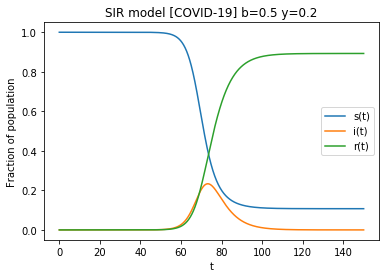
\includegraphics[width=9cm]{img/covidb12y15.png}
\centering
\caption{COVID-19 in SIR Model for $\beta=0.5$}
\label{fig:covid1}
\end{figure} 


But if we decrease the number of infections to one per 5 days, so the $\beta = 0.2$, then there is no epidemic:

\begin{figure}[ht]
    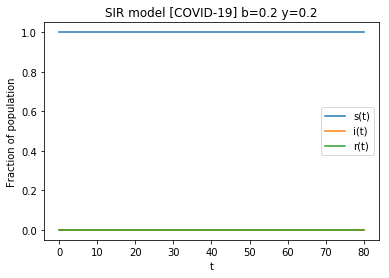
\includegraphics[width=9cm]{img/covidb15y15.png}
    \centering
    \caption{COVID-19 in SIR Model for $\beta=0.2$}
    \label{fig:covid3}
\end{figure} 

We can easly notice that, the factor determining if the epidemic will happen is the rate of new infections $\frac{di}{dt}$, if it is positive, then there will be epidemic, and if it's negative, people will recover faster than spread of infection, so there will be no epidemic.

We can calculate the value of $\frac{di}{dt}$ in the $t_0$ and check if the value is negative of positive, the negative value mean the decrease of infections from the beginning, so we can be sure that, there will be no infections.

Let's represent the factor determining of the epidemic in form of inequation, which if satisfied, will lead to epidemic

\[i(t) \beta s_0 - \gamma i(t) > 0\]

Since the fraction of infections $i(t)$ is never negative, we can omit it in our inequation.

\[\beta s_0 - \gamma > 0\]
\[ s_0 > \frac{\gamma}{\beta}\]

Here we can introduce $R_0$ as Basic Reproduction Number

\[ R_0 = \frac{s_0 \beta}{\gamma}\]

which represent the number of people, each infected person can infect before being recovered. Thus if $R_0 = 2$ then each infected person can infect on average 2 new people before being recovered, so the number of infections grows exponentially, and if $R_0 = 0.5$, then for each 2 people, only 1 new infection happens, and the number of infections decrease exponentially. $R_0 = 1$ is called $epidemic threshold$ where the number of new infections equals the number of recovers, so the total number of infected people is always the same and equals the initial number of infected people $I_0$. For example, the Basic Reproduction Number $R_0$, for seasonal flu the value is estimated between 0.9–2.1\cite{coburn2009modeling}, whereas for COVID-19 it's estimated to 2.2 in early stage (January) \cite{li2020early} and recently to 5.7 (April) \cite{readeid}.

To decrease the results of epidemic, we can decrease the numbers $s_0$ and/or $\beta$, or increase $\gamma$. Since we have little control over the time of recovery ($\gamma$), the only way to reduce the impact of infection is to reduce the number of contact between infected and suspicious people. That's why, the social distancing is so important in fight with epidemics.


It might be also valuable to know the maximum number of infected people at any given time. We can calculate it by combining the first two parts of SIR differential equations.
\[
\begin{rcases}
\frac{dS}{dt} = - I \beta S \\
\frac{dI}{dt} = I \beta S - \gamma I
\end{rcases}
\]

into 

\[\frac{dI}{dS} = \frac{\beta I S - \gamma I}{\beta I S}\]

which then reduces to 
\[\frac{dI}{dS} = -1 + \frac{\gamma}{\beta S}\]

here we can replace $\frac{\beta}{\gamma}$ by $q$; so called \textit{contact ratio}, which is described as fraction of population, that comes into contact with an infected individual, during the period when they are infectious.

\[\frac{dI}{dS} = -1 + \frac{1}{q S}\]

now we can integrate the equation and get

\[I + S - \frac{1}{q} \ln{S}\]

then we apply the initial conditions and get the equation:

\[I + S - \frac{1}{q} \ln{S} = I_0 + S_0 - \frac{1}{q} \ln(S_0)\]

We know that to find the function maximum we need to find the place where its deritive equals zero. And here, the right side of the equation 

\[\frac{dI}{dS} = -1 + \frac{1}{q S}\]

equals to zero, when this equation is satisfied.

\[1 = \frac{1}{q S}\]

which happens when 

\[S = \frac{1}{q}\]

In order to find the maximum value of I, we can replace the $S$ by $\frac{1}{q}$ in the equation

\[I + S - \frac{1}{q} \ln(S) = I_0 + S_0 - \frac{1}{q} \ln(S_0)\]

so we get

\[I_{max} + \frac{1}{q} - \frac{1}{q} \ln(\frac{1}{q}) = I_0 + S_0 - \frac{1}{q} \ln(S_0)\]

\[I_{max} = - \frac{1}{q} + \frac{1}{q}\ln(\frac{1}{q}) + I_0 + S_0 -\frac{1}{q}ln(S_0)\]

\[I_{max} = I_0 + S_0 - \frac{1}{q} ( 1 - \ln(\frac{1}{q}) + ln(S_0))\]

\[I_{max} = I_0 + S_0 - \frac{1}{q} ( 1 + \ln(q S_0))\]

For example we can calculate the $I_{max}$ for our COVID-19 example 

\[I_0 = 3 \quad S_0 = 7.8 * 10^9 \quad R_0 = 0\]

\[\beta = 0.5 \quad \gamma = 0.2 \quad q = 2.5\]

\[I_{max} = 3 + 7.8 * 10^9 - 0.4 ( 1 + \ln(2.5 * 7.8 * 10^9))\]

\[I_{max} = 1 - 0.2/0.5 * (1 + ln(0.5/02 * 1)) = 0.233\]
Which, based on the total population of the world would result in maximum of $7.8 * 10^9 * 0.233 = 1.8 * 10^9$ infected people at a time.

We can plot function $f(\beta)$, and see how parameter $\beta$ influences the maximum number of infectious fraction of population at a given time. For readability we use log scale.

\begin{gnuplot}[scale=0.8]
    set title '$I_{max}(\beta)$ for $\gamma=0.2$'
	set ylabel '$f(\beta)$'
	set xlabel '$\beta$'
	set logscale x
	gamma = 0.2
	f(x) = 1 - gamma/x * ( 1 + log(x/gamma))
	plot [0.2:100] f(x) notitle
\end{gnuplot}

We can see that at first the value grows exponentially, but then saturates similar to "logistic growth function". The value 1.0 (whole population is infected at a time) can not be achieved using this model, because

\[I_{max} = 1 = 1 - 0.2/\beta * (1 + \ln(\beta/0.2))\]

would require either 

\[0.2/\beta = 0\]

or 

\[\ln(\beta/0.2) = -1\]

which will never happen. 
Theoretically, the time period between first recovery (which we estimated on about 5 days) would make it possible to infect whole population before anyone gets recovered (assuming small population, or enormous contact ratio)

\subsection{SIS Model}

There are some kind of diseses, where the individual can gets infected many times e.g. the flu. Therefore there is no Recovered population. This could be because of the disese is mutating or the antibody doesn't persist long enough in the organism. For this kind of epidemic, the state flow looks following $Suspicious -> Infected -> Suspicious$, hence the name SIS. 
To calculate this kind of model, we need modify the previous equations, that the change $\gamma i(t)$, will go to suspicious state, instead of recovery.

\[\frac{si}{dt} = - i(t) \beta s(t) + \gamma i(t)\]

\[\frac{di}{dt} = i(t) \beta s(t) - \gamma i(t)\]

with

\[ s + i = 1\]

we can solve the equation by substituting $s$ in second equation, and solving Linear Differential Equations

\[\frac{di}{dt} = i(t) * \beta * (1 - i(t)) - \gamma * i(t)\]

After integrating the solution is:

\[i(t) = (1 - \frac{\gamma}{\beta}) \frac{C}{C + e^{-(\beta - \gamma)t}}\]
where 
\[C = \frac{\beta i_0}{\beta-\gamma-\beta i_0}\]

we can plot the function $i(t)$ for constant $\gamma = 0.2$ and $\beta = 0.5$

\begin{gnuplot}[scale=1]
    set title '$i(t)$ for $\beta = 0.5$ and $\gamma=0.2$'
    set ticslevel 0.0

	set xlabel '$days$'
	set ylabel '$i$'

    set xrange [0:100]
    
	gamma = 0.2
	beta = 0.5
	i0 = 3.8 * 10**(-10)
	
	c(b) = (b*i0)/(b-gamma-b*i0)
	f(x) = (1 - gamma/beta) * (c(beta))/(c(beta) + exp(-(beta-gamma)*x))
	plot f(x) notitle
\end{gnuplot}

we can also plot the function $i(t, \beta)$ for constant $\gamma = 0.2$ and see how the $\beta$ influence the results.

\begin{gnuplot}[scale=1]
    set title '$i(\beta,t)$ for $\gamma=0.2$'
    set ticslevel 0.0
    
	set xlabel '$\beta$'
	set ylabel '$t$'
	set zlabel '$i$'
	set ztics 0,1.0
	
	set view 45,315
	
    set xrange [0.1:0.8]
    set yrange [0:1000]
    
    set isosamples 50,50
    

	gamma = 0.2
	i0 = 3.8 * 10**(-10)
	
	c(b) = (b*i0)/(b-gamma-b*i0)
	f(x,y) = (1 - gamma/x) * (c(x))/(c(x) + exp(-(x-gamma)*y))
	splot f(x,y) notitle
\end{gnuplot}


As we can see, the logistic growth S-curve shape of the number of infected population is driven by the $\beta$ factor. If the value is less than $\gamma$, the epidemic never occur. Values greater than $\gamma$ lead to constant fraction of infectious population (rate of catching the infection by suspicious population is equal to rate of recovers in infected population). The higher the value, the faster the outbreak comes out, and the higher the infection ratio holds.

\subsection{SIRS and SEIRS Models}
SIRS model introduces another state change, allowing the recovered people to lose their immunity to the infection. Therefore the state flow looks following: $Susceptible -> Infected => Recovered -> Susceptible$. Luckly, we can write the equations for this model, by simply adding one intermediete state equation to the SIS equations.

\[\frac{si}{dt} = \delta r(t) - i(t) \beta s(t)\]

\[\frac{di}{dt} = i(t) \beta s(t) - \gamma i(t)\]

\[\frac{dr}{dt} = \gamma i(t) - \delta r(t)\]


Another, more complex model in terms of states is the SEIRS model. This model introduces ihe intermediary state between susceptable and infected state. The \bold{E}xposed is the state, where the individual is infected, but is not spreading the infection to other people. Such modification is also easy to write by adding another intermiediary state to previous SIRS model accordingly.

\[\frac{si}{dt} = \delta r(t) - i(t) \beta s(t)\]

\[\frac{ei}{dt} = i(t) \beta s(t) - \gamma e(t)\]

\[\frac{di}{dt} = \gamma e(t) - \omega i(t)\]

\[\frac{dr}{dt} = \omega i(t) - \delta r(t)\]

As we can see, those modes can be easly extended to infinite number of intermediary states, more accurately reflecting the reality. Unfortunately there is not known analytical solution to such models, we have to solve them by numerical integration of  differential equations.

\subsection{Summary}
Those models operate on idealistic full-mixing assumption, where each individual has equal probability to contact anyone else. This assumption doesn't reflect exactly the human interaction nor computer networks. It's rather approximation, the parameter $\beta$ reflects the chance that individual will have contact with someone else and the infection will spread. In our problem, the network is static, the structure of nodes is fixed, each node has unique set of neighbours where the disease can spread. In real life this might be the family members, friends or coworkers. The chance of contact with the rest of the population can be neglected, because the chance of meeting two people from two end of the earth is very small. For this reason we have to create different model of infection dissemination. 

In our model the infection is the abstract, representing trust to an content. We should take a look how the trust graph are build to understand how we could leverage the mechanisms for our infection spread.


\section{Trust graph}
\label{trust-graph}
%ow are they created ? In life, in networks ? What does it mean to create trust relationship. What do we understand by trust relationship. In environments that or another. 

%Then we assume that such relation is already achieved. LOCKSS - solve the problem in one way, Wikipedia in another (experts consensus), but they doesn't fit to us, why ?. 

Why do we even look for solution for our problem in the context of human trust ? It turns out that people are still one of the most advanced technology. We can get inspired by some of the solutions that works in human societies for centuries. Let's dive into it.
Yuval Noah Harari in his book "Sapiens: A Brief History of Humankind" \cite{harari2014sapiens} states that the most important feature of human language is rumor. Rumor let us know which person is not trustworthy without having to interact with him directly. If our best friend Bob, tells us, that Carlie is theft, we don't need to get stolen to be convinced about it. Same applies in inverse scenario, if Bob tells us, that Carlie sells great quality products, we are now more likely to buy products from him; we are biased towards people, whom we gets positive rumors. We notice that each person we know directly or indirectly, gets labeled with some tags. One can be labeled as Helpful, Conscientiousness and also Not-Trustworthy, while other can be labeled as Unhelpful, Lazy but Trustworthy. Here in this paper, we are limiting our range of study just to dimension of Trustworthness.
What if we have three friends Alice, Bob, Charlie. Alice and  Bob tells us that David is Trustworthy, while Charlie claims that he's not. Decision of labeling David as Trustworthy or not, requires some kind of decision evaluation algorithm.
One might assume that if there is at least one person who doesn't trust him, there must be something wrong with him, and will label him as Not-Trustworthy. One can use the most natural to human beings evaluator which says, do want majority of people do, thus if Charlie is trusted by majority, I will trust her too. Another one can slightly generalise this evaluator and say that person is trustworthy, only if $\xi$ percentage of my friends trust him. 

At this point it's worth introducing some convention. When we say friend we mean a trustworthy person, in other words, person who we have trust relation to. Let $N$ to be a set of all considered individuals group, friends and non-friends. Let $F$ be a set of all our friends $f \in F$. Let $F_n$ be a subset of $F$ where all $f$ trust person $n$. Then we will call $\%_n = |F_n|/|F|$ the proportion of our fiends who trust particular person $n$. Let's call $\xi$ (where $0 \le \xi \leq 1$) the minimum proportion of our friends $\%_n$ who needs to trust person $n$ in order to make me trust him. 

So as we said previously that we will trust David only if majority of our friends trust him. We denote trust function as $T(n) = \%_n > \xi : (N) \rightarrow \{0,1\}$. 
Let's use this formula to evaluate if $David$ is trustworthy person. Let $\xi = 0.5$. We know that Alice and Bob does trust David, while Charlie doesn't.
\[T(David) = \%_{David} > \xi\]
\[= |F_n|/|F| > \xi\]
\[= \frac{2}{3} > \frac{1}{2}\]
Then it turns out that $David$ is \textbf{Trustworthy}


People with low $\xi$ easly gets manipulated, we call them naive.
People with high $\xi$ hardly gets convinced, we call them stubborn. 

Another generalisation might be adding weights to this evaluator, let's say that Charlie is our brother, while Alice and Bob are our cousins, and we trust 3 times stronger to our brother than cousin. Let's call $W(f): (F) \rightarrow \Re$ the function that maps our friend to the weight of how strong we trust him. In this case weighted proportion of our friends \[\%_n = \frac{\sum\limits_f^{F_n} W(f)}{\sum\limits_f^{F} W(f)}\]

When we assume weights $W(Alice) = 1, W(Bob) = 1, W(Charlie) = 3$, and $\xi = 0.5$. We can calculate weighted proportion $T(David)$ as follows:
\[T(David) = \%_n > \xi\]
\[= \frac{\sum\limits_f^{F_n} W(f)}{\sum\limits_f^{F} W(f)} > \xi\]
\[= \frac{\sum \{1,1\}}{\sum\{1,1,3\}} > \frac{1}{2}\]
\[= \frac{2}{5} > \frac{1}{2}\]
Then it turns out that $David$ is \textbf{Not-Trustworthy}

But this view is based on static network of connections. We somehow meet Alice, Bob and Charlie, and we gets convinced about their trustworthness. Thus there must be a second way of gaining our trust. Let's modify our trust function by allowing External Trust Obtaining(ETO). $T(n) = \%_n > \xi \lor ETO(n) : (N) \rightarrow \{0,1\}$.

Another think we can observe in the context of trust network is time. Should we still trust our friend from elementary school if we haven't seen him for decades ? We could modify the trust function to be dependent on the time, but for now let's assume that the friendship is immortal.

Next, if we have a friend, who have a friend, we will trust that person. But if someone ask us, if that person is our friend, we will say no. Therefore only the friendship relation can propagate the trust.

Having the trust network model, we can try to simulate the epidemics using the graphs obtained by that model. Let's describe the algorithm used to generate trust graphs.
We start with the $N_0$ nodes that gets connected with random $E_0$ edges. They becomes the root of the friendship. Each of them meets new people, and becomes friends. So for all remaining $N - N_0$ nodes we connect to one randomly selected node with friend relation. The new node $N_n$ connect to the old node $N_o$ then, for all $N_o$ friends $F_{N_o}$ we need to evaluate the trust function $T(n)$.

In Fig \ref{fig:trustgraph500} we can see the resulting trust graph for 500 nodes and $\xi = 0.5$, and its corresponding histogram in \ref{fig:trustgraph500histogram}

\begin{figure}[h!]
    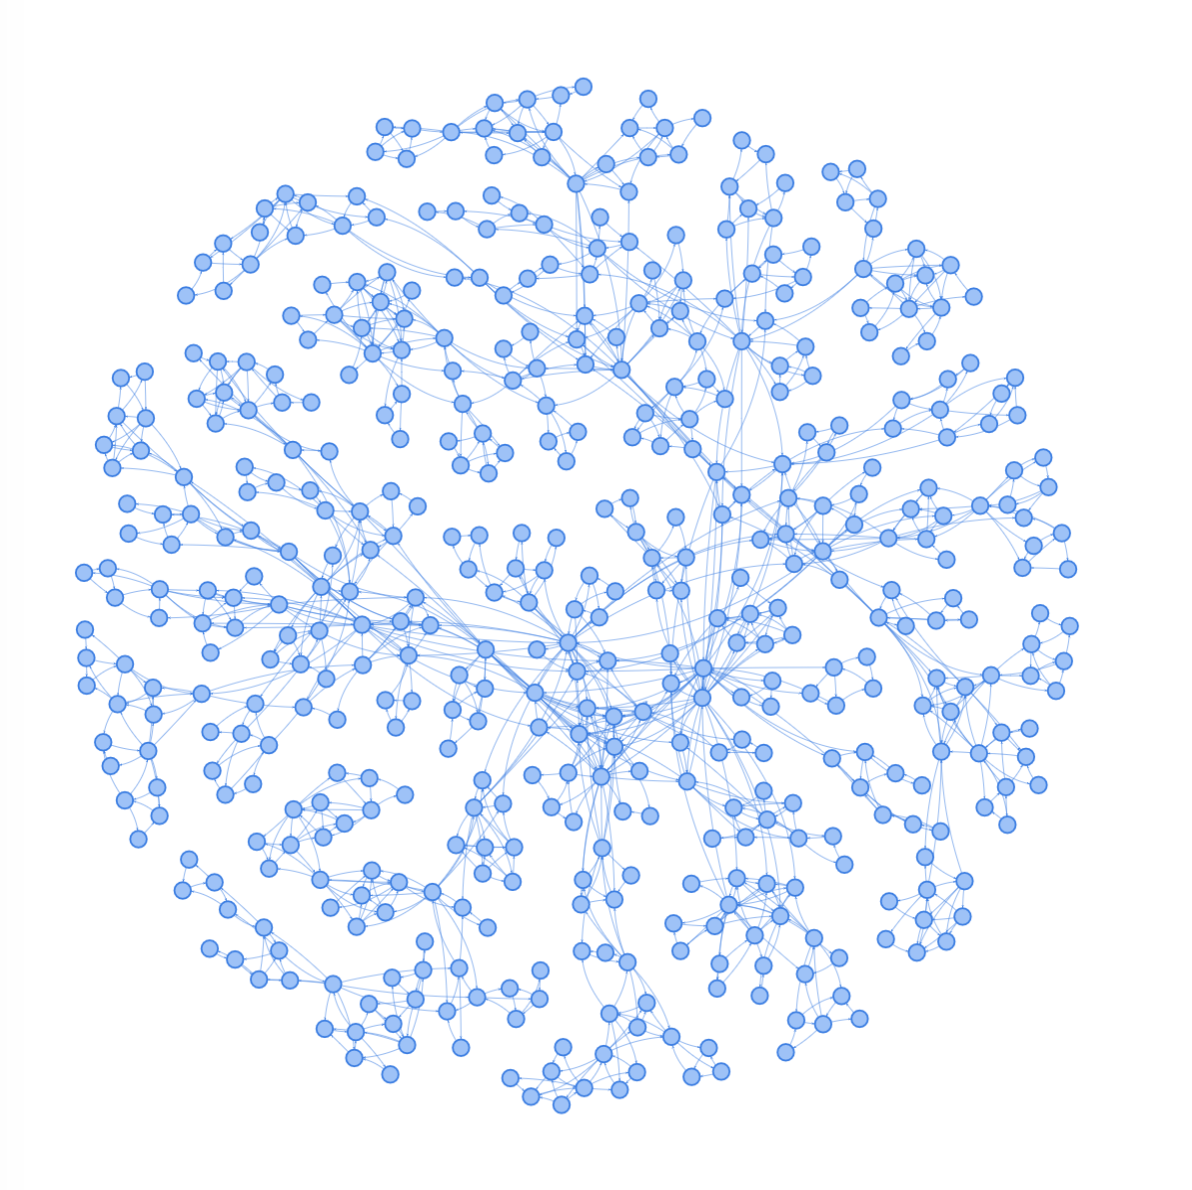
\includegraphics[width=11cm]{img/webOfTrust500Graph.png}
    \centering
    \caption{Trust Graph generated by Web Of Trust algorithm for $\xi=0.5$ and $n = 500$}
    \label{fig:trustgraph500}
\end{figure}

\begin{figure}[h!]
    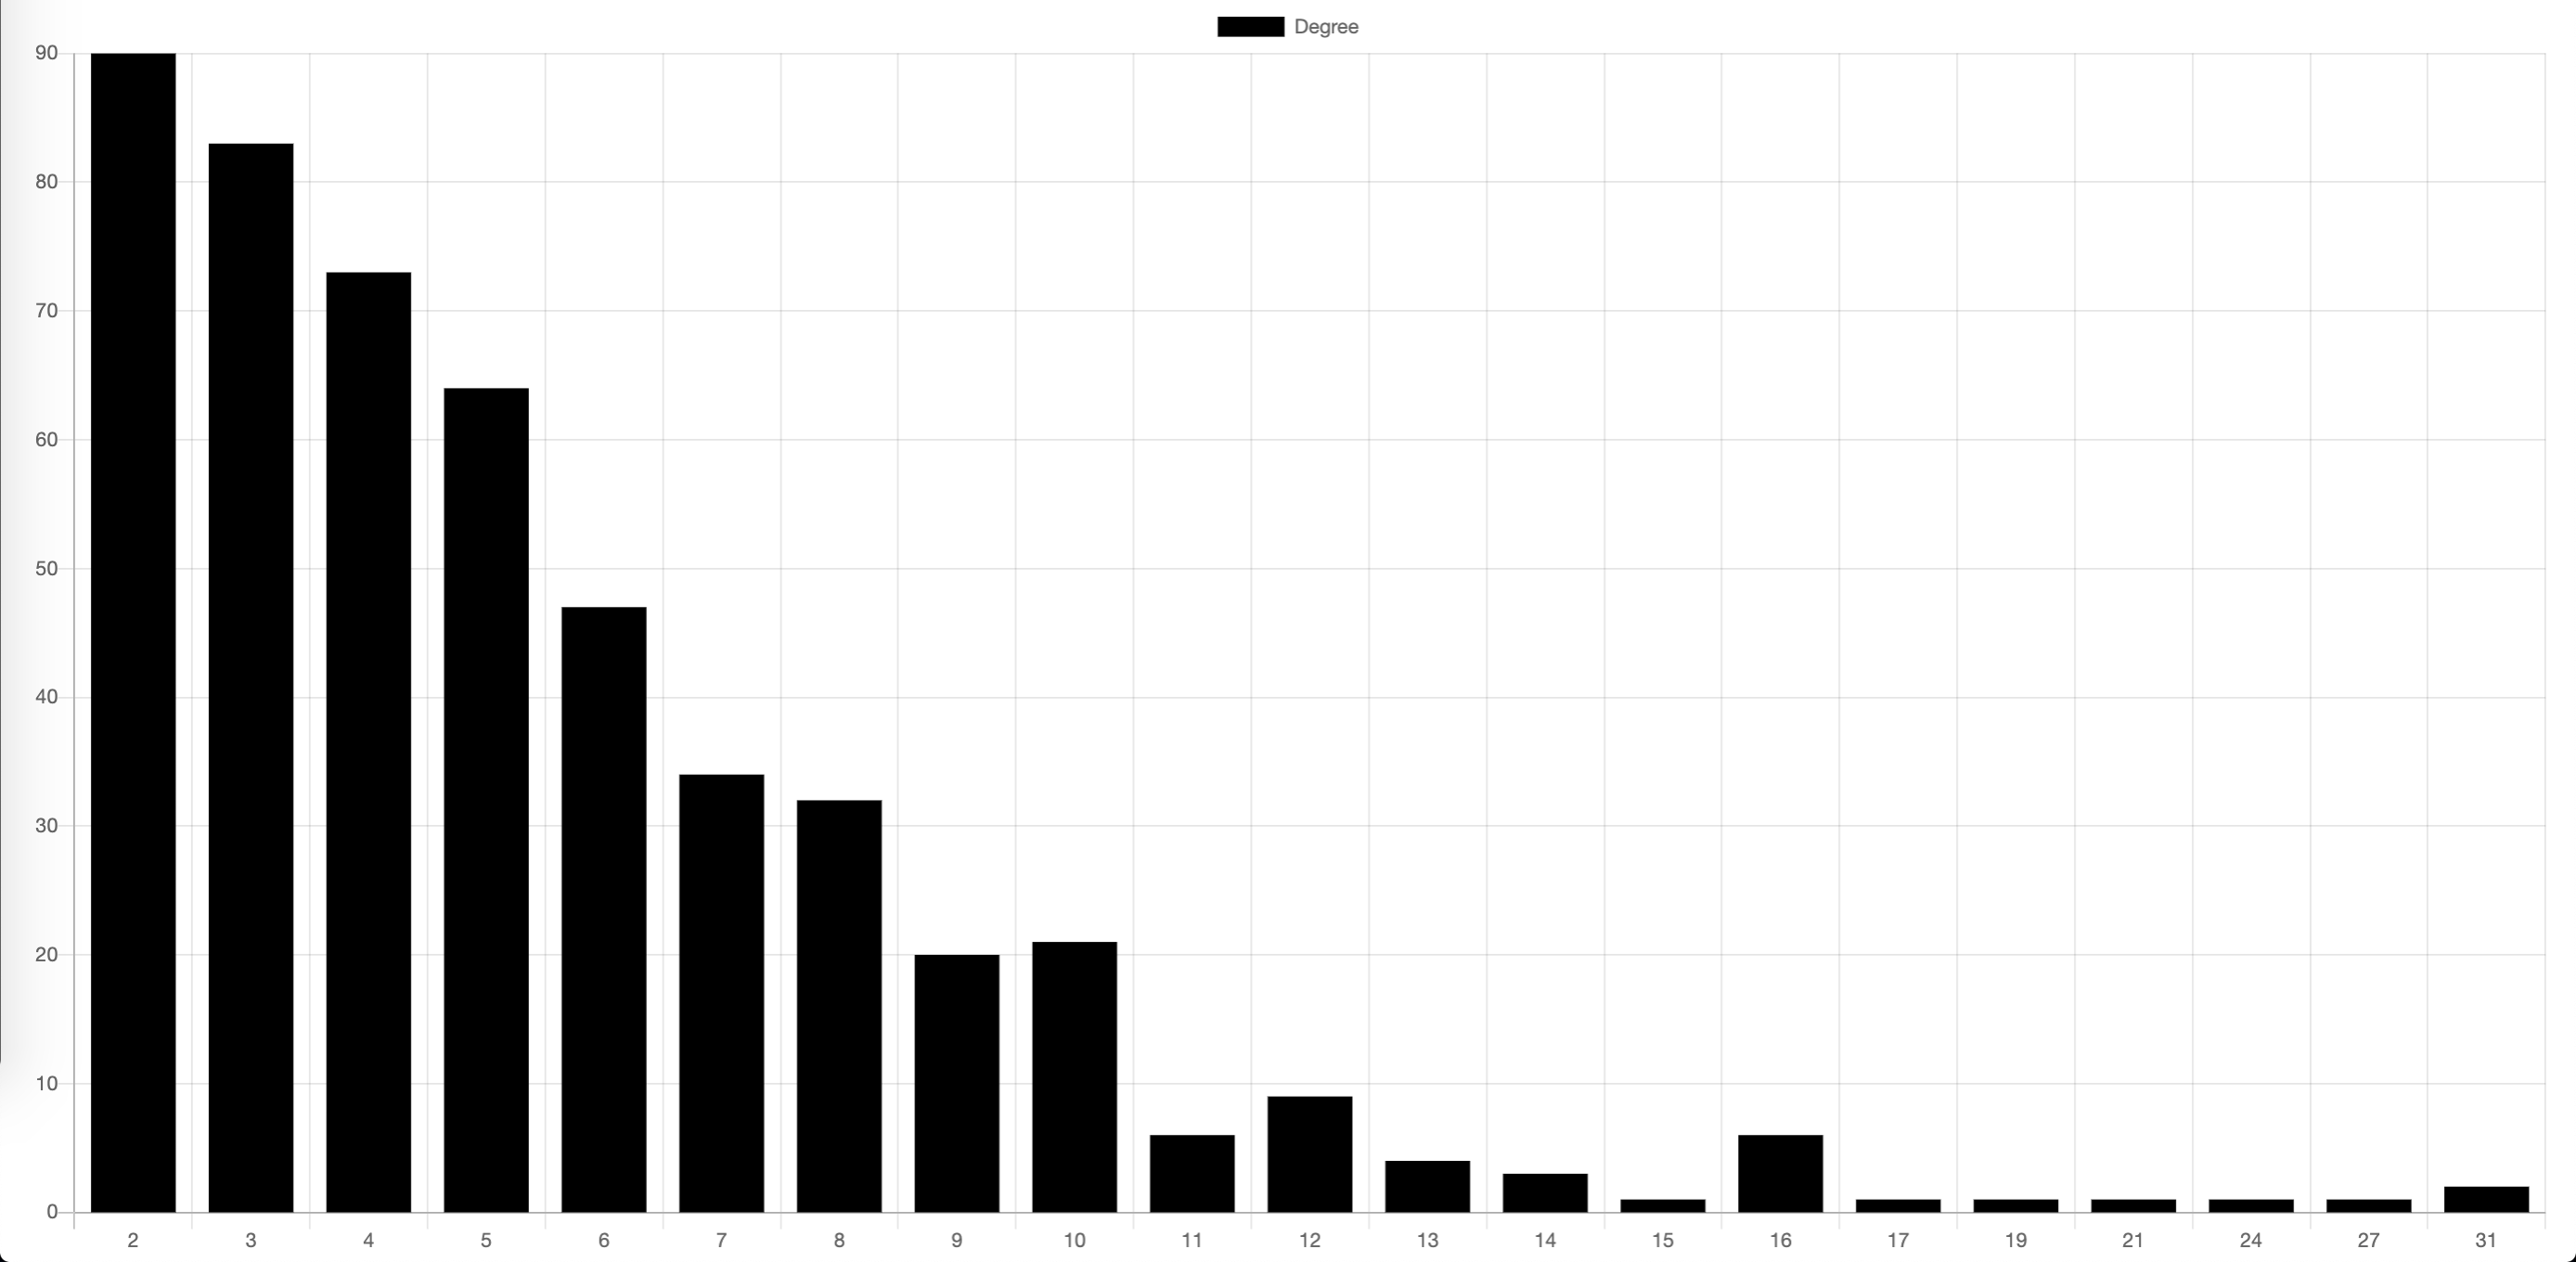
\includegraphics[width=11cm]{img/webOfTrust500Hist.png}
    \centering
    \caption{Degree Histogram generated by Web Of Trust algorithm for $\xi=0.5$ and $n = 500$}
    \label{fig:trustgraph500histogram}
\end{figure} 

\subsection{Different types of trust graph generators}
\paragraph{Random generator}
Random graph generation is the simplest one. We take n nodes, m edges -- each edge is connected to two random nodes $n_1$, $n_2$ where $n_1 != n_2$. Although random trust graph is far from reality, we will use it for comparison.

\paragraph{Probabilistic duplication}
Another trust graph generator proposed in \cite{konorski2019mitigating} base on probability duplication and can be visualized as natural process of acquiring new colleagues on our friends' party. When we get to the party, we meet new people who with some probability become our colleagues. This algorithm works as follows: we take initial $n_0$ nodes and $m_0$ edges and connect them randomly---creating kernel. Then we add new node and connect it to one random node in current graph (your friend invited you to his party), then with $\phi$ probability you connect to each of his friends (you acquire new friends with some of his friends), you repeat this process $n = N - N_0$ times. 
The most important advantage of this generator is the fact that it produces scale-free graphs. Figure \ref{fig:propdup500graph} shows the graph generated by the method and Figure \ref{fig:propdup500histogram}, histogram of edge degrees.

\begin{figure}[h!]
    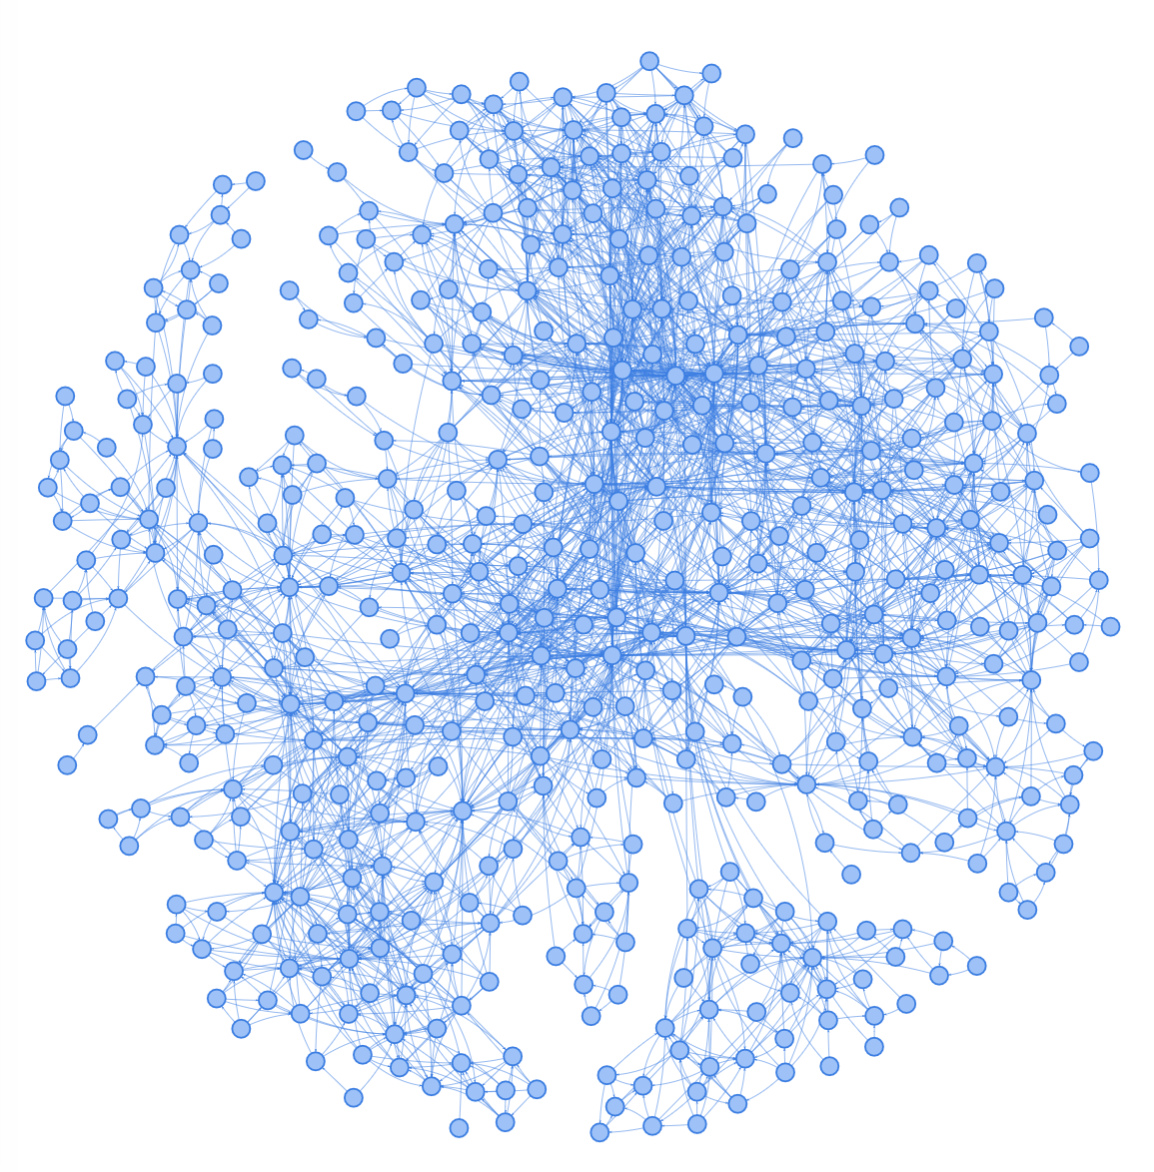
\includegraphics[width=11cm]{img/propDup500Graph.png}
    \centering
    \caption{Trust Graph generated by Probabilistic Duplication algorithm for $\xi=0.5$ and $n = 500$}
    \label{fig:propdup500graph}
\end{figure}

\begin{figure}[h!]
    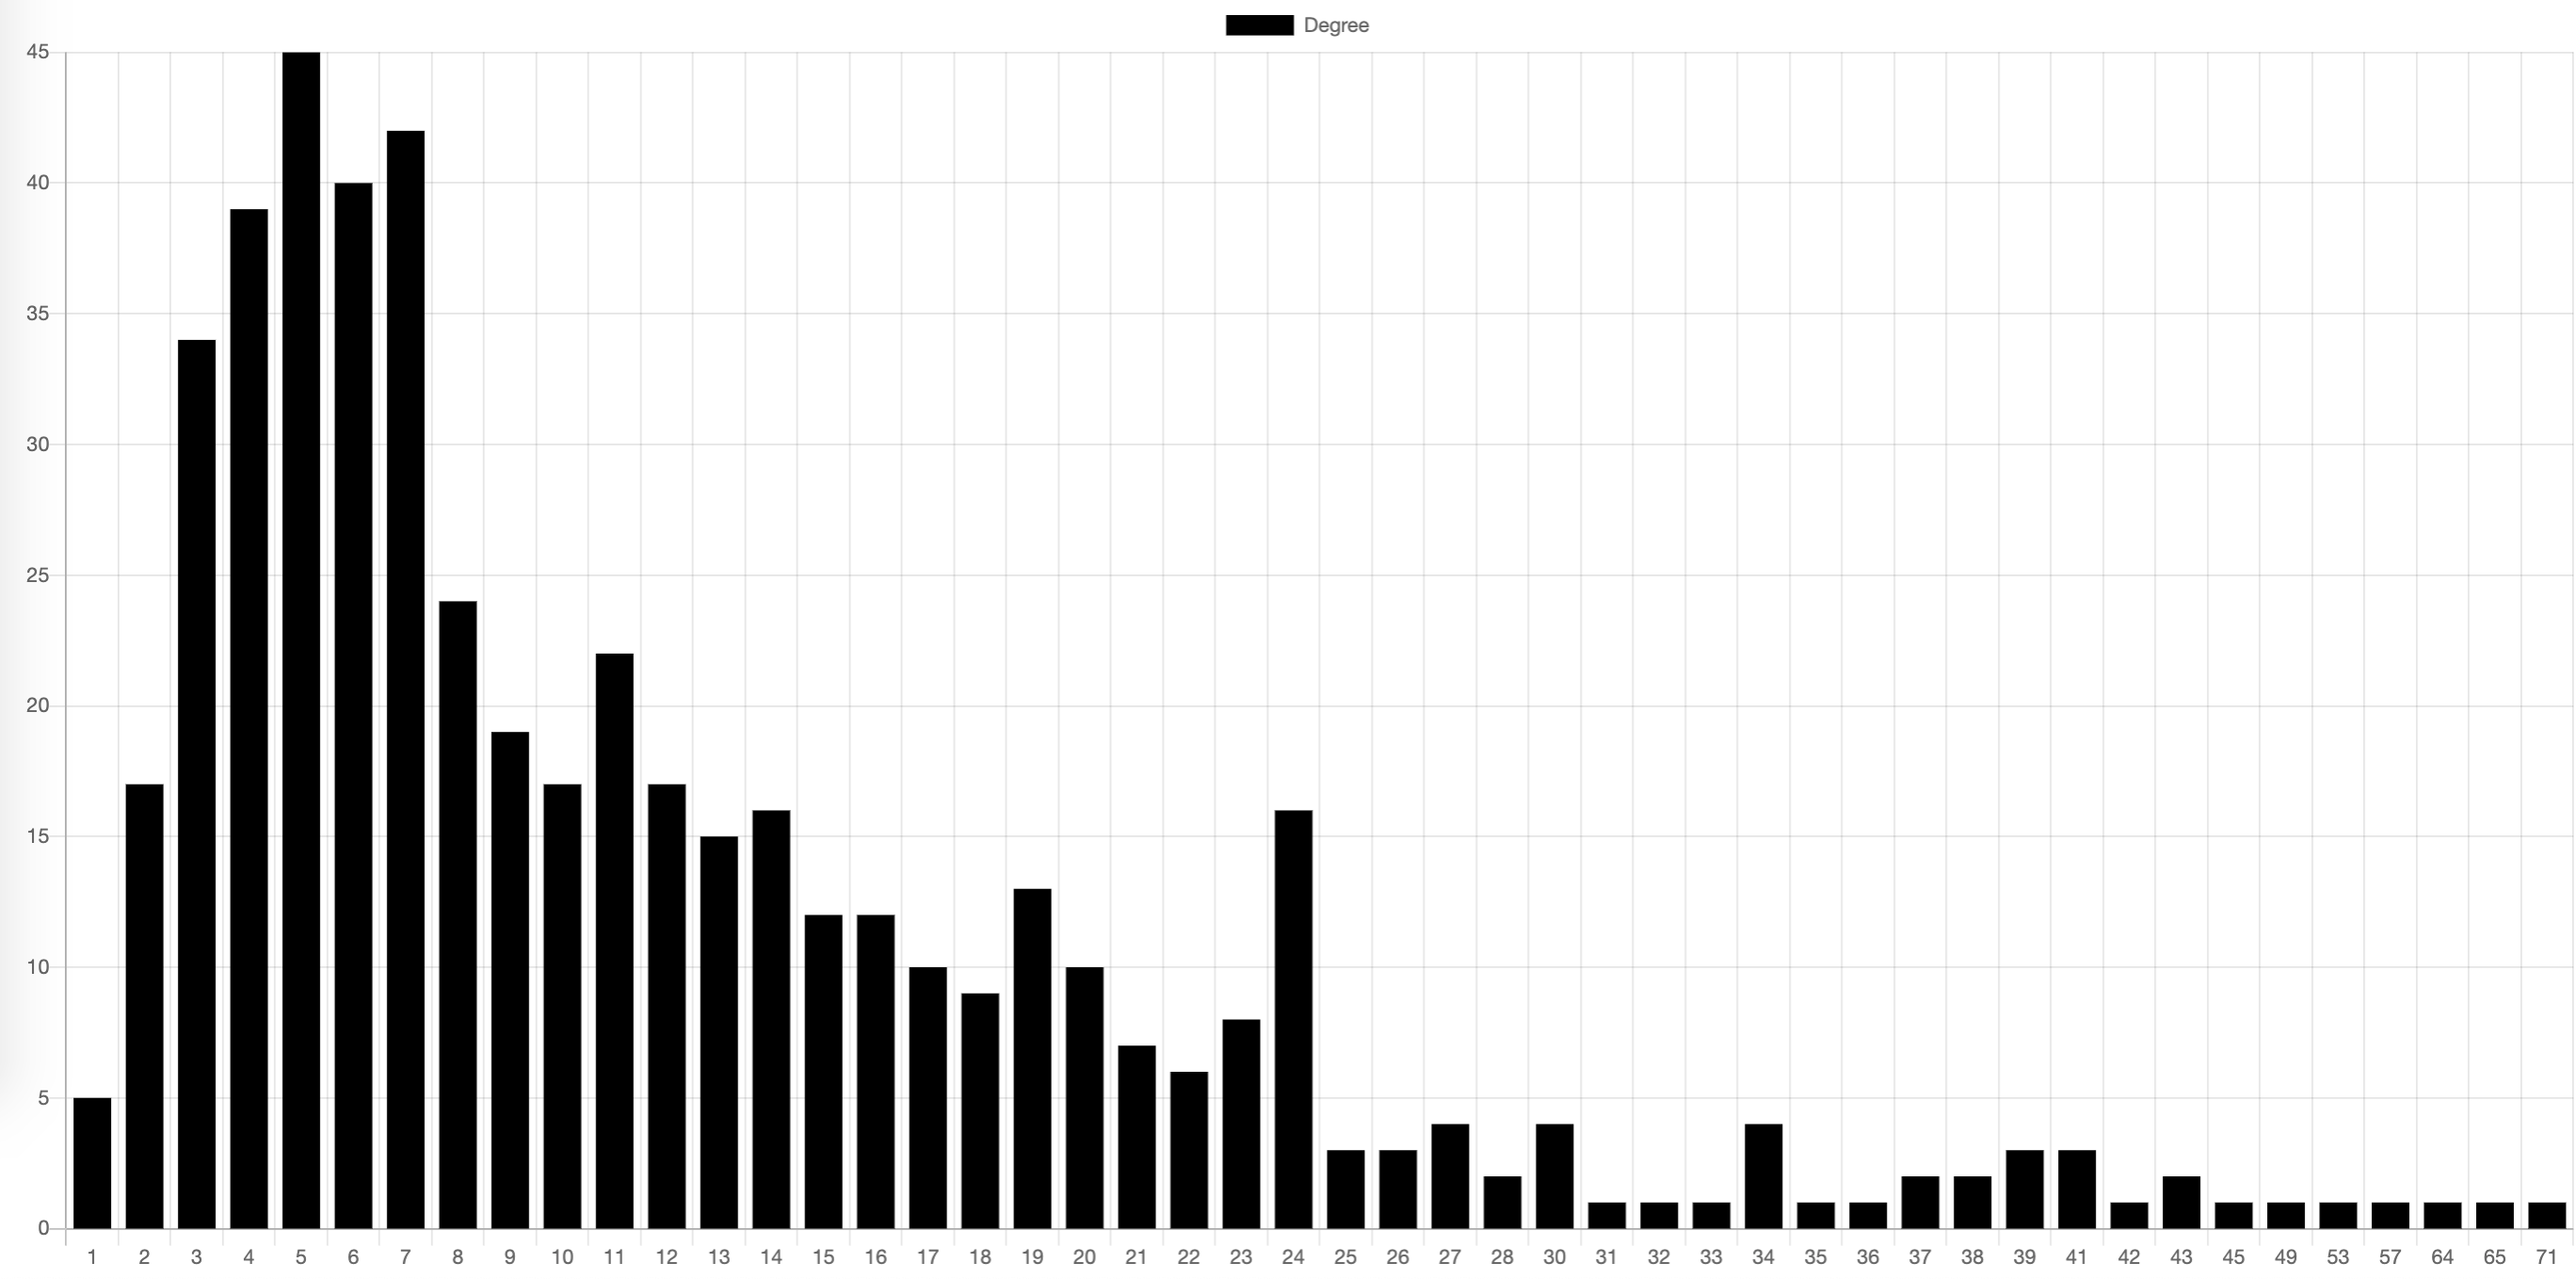
\includegraphics[width=11cm]{img/propDup500Hist.png}
    \centering
    \caption{Degree Histogram generated by Probabilistic Duplication algorithm for $\xi=0.5$ and $n = 500$}
    \label{fig:propdup500histogram}
\end{figure} 

\section{Stolen Credentials Problem}
ICN authentication model is based on credentials.  Unit with access to credentials can publish authenticated data, because rest of the network has no other ways to verify the content authentication other than checking signature validity (created with credentials). Credentials can be loosely categorized to two categories: cold/offline credentials e.g. private keys -- this type of credentials has very long (days or months) or not at all expiration time, they are typically stored on hard drives and rarely leave the device; hot/online credentials e.g. access tokens -- are created for limited period of time(minutes or hours) and are often transmitted over the network. 
Stolen Credentials is serious problem. Multi-factor authentication methods tries to mitigate the problem, but here in this thesis we assume that even it -- is not able to stop such attacks.
Stolen credentials in conjunction with ICN caching, can lead to destructive consequences, because ICN protocols doesn't provide data revoking/removal functions. Malicious entity who gains access to stolen credentials can publish authenticated data that can stays in nodes' cache for long(how long) period of time. 

For cold/offline data breaches we can find reports (DBIR - Data Breach Investigations Report 2020) showing that 45\% of attacks is caused by "hacking", 22\% is caused by misconfiguration, 22\% by phishing.  17\% caused by malicious software, 4\% by misuse by authorized users and 4\% by physical interaction.

Most of the attacks (70\%) are performed by external entities, who are financially motivated (86\%), also most attacks are targeted on big corporations (72\%). In most of them (58\%) the data breach include users personal informations.  

If we look at historical data in Fig. \ref{fig:data-breach-historical}.
\begin{figure}[h!]
    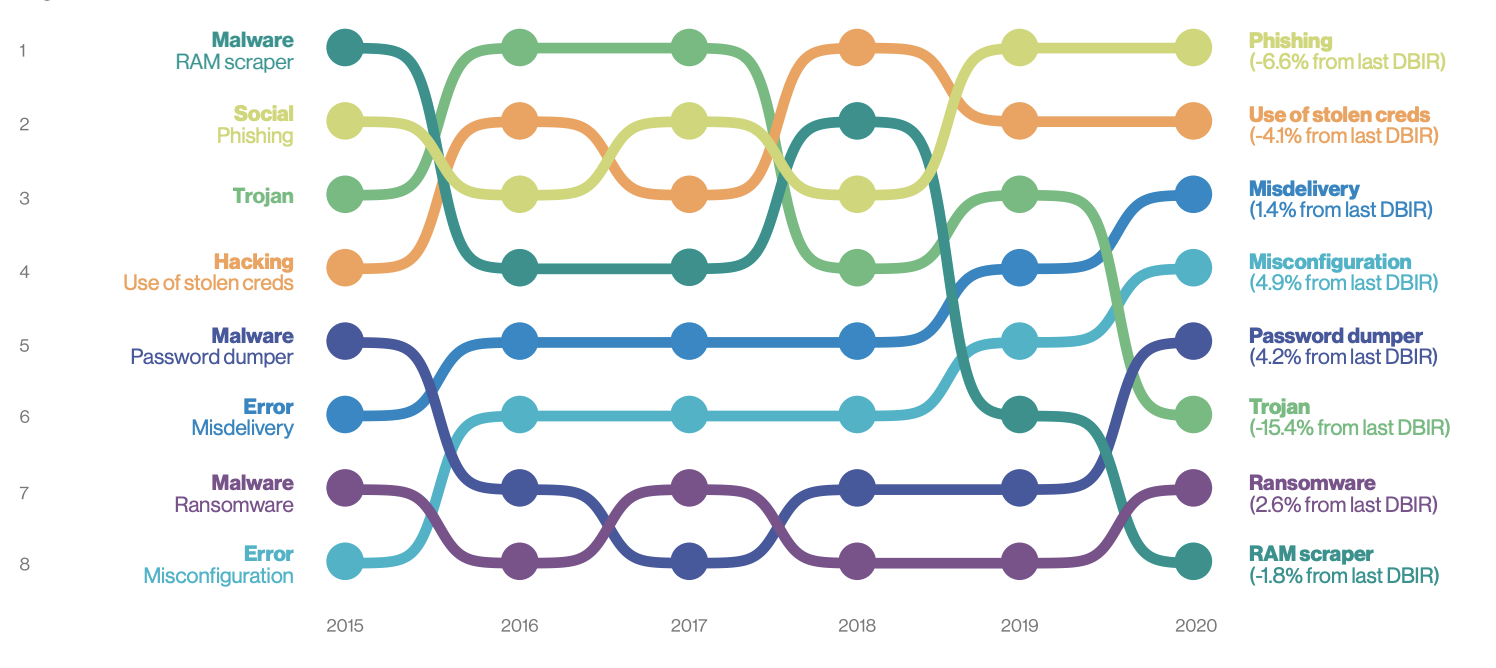
\includegraphics[width=1\textwidth]{img/data-breach-historical.png}
    \centering
    \caption{Select action varieties in breaches over time. Source: Data Breach Investigations Report 2020}
    \label{fig:data-breach-historical}
\end{figure} 
The most decrease gets Trojan horses -- from 50\% in 2016 to 5.6\% in 2020. Similar decrease gets RAM Scrapers, which search operating system memory for potential confidential data. 
On contrary, the highest increase can be noted on misconfiguration and accidental data leakage. Yet the highest popularity is still for phishing attacks and usage of stolen credentials. 
In fig \ref{fig:credentials-steal-discovery}, we can see that for 60\% of incidents, \textit{the breach was discovered in less than one day}, and the trend is increasing -- more incidents are discovered in less than one day. For 25\% of incidents, the incidents were discovered in one or more months. But, it must be noted that some of the breaches might not be discovered yet, so the value might be underestimated. In this report, we can find that the number of discoveries increased due to Managed Security Service Providers (MSSP), which are obligated to publish such breach incidents.

\begin{figure}[h!]
    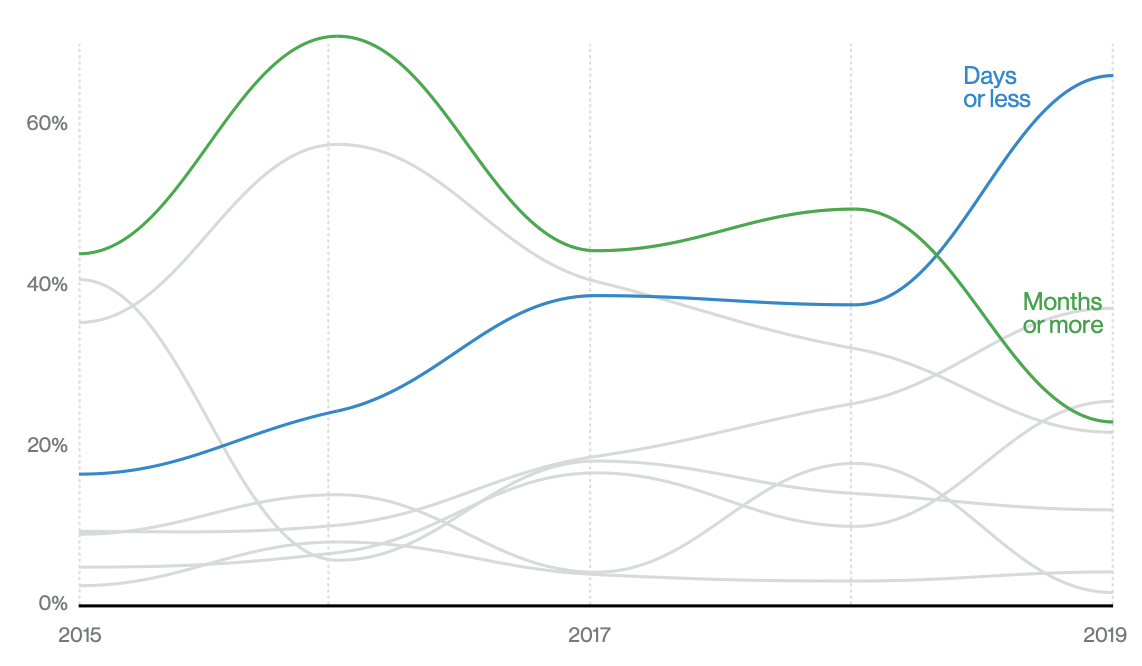
\includegraphics[width=11cm]{img/credentials-steal-discovery.png}
    \centering
    \caption{Discovery over time in data breaches. Source: Data Breach Investigations Report 2020}
    \label{fig:credentials-steal-discovery}
\end{figure} 


For hot/online credentials 
%TODO
//TODO


\section{Graph Infections}
Graph Infection algorithm proposed in \cite{konorski2019mitigating} is similar to SEIRS model, but some changes were made. The possible node states are \textbf{S}usceptible-\textbf{A}cute-\textbf{R}ecoverable-\textbf{Q}uarantine-\textbf{S}usceptable (SARQS), the flow diagram is presented in fig. \ref{fig:finite-state-machine-jekon}.
\begin{figure}[h!]
    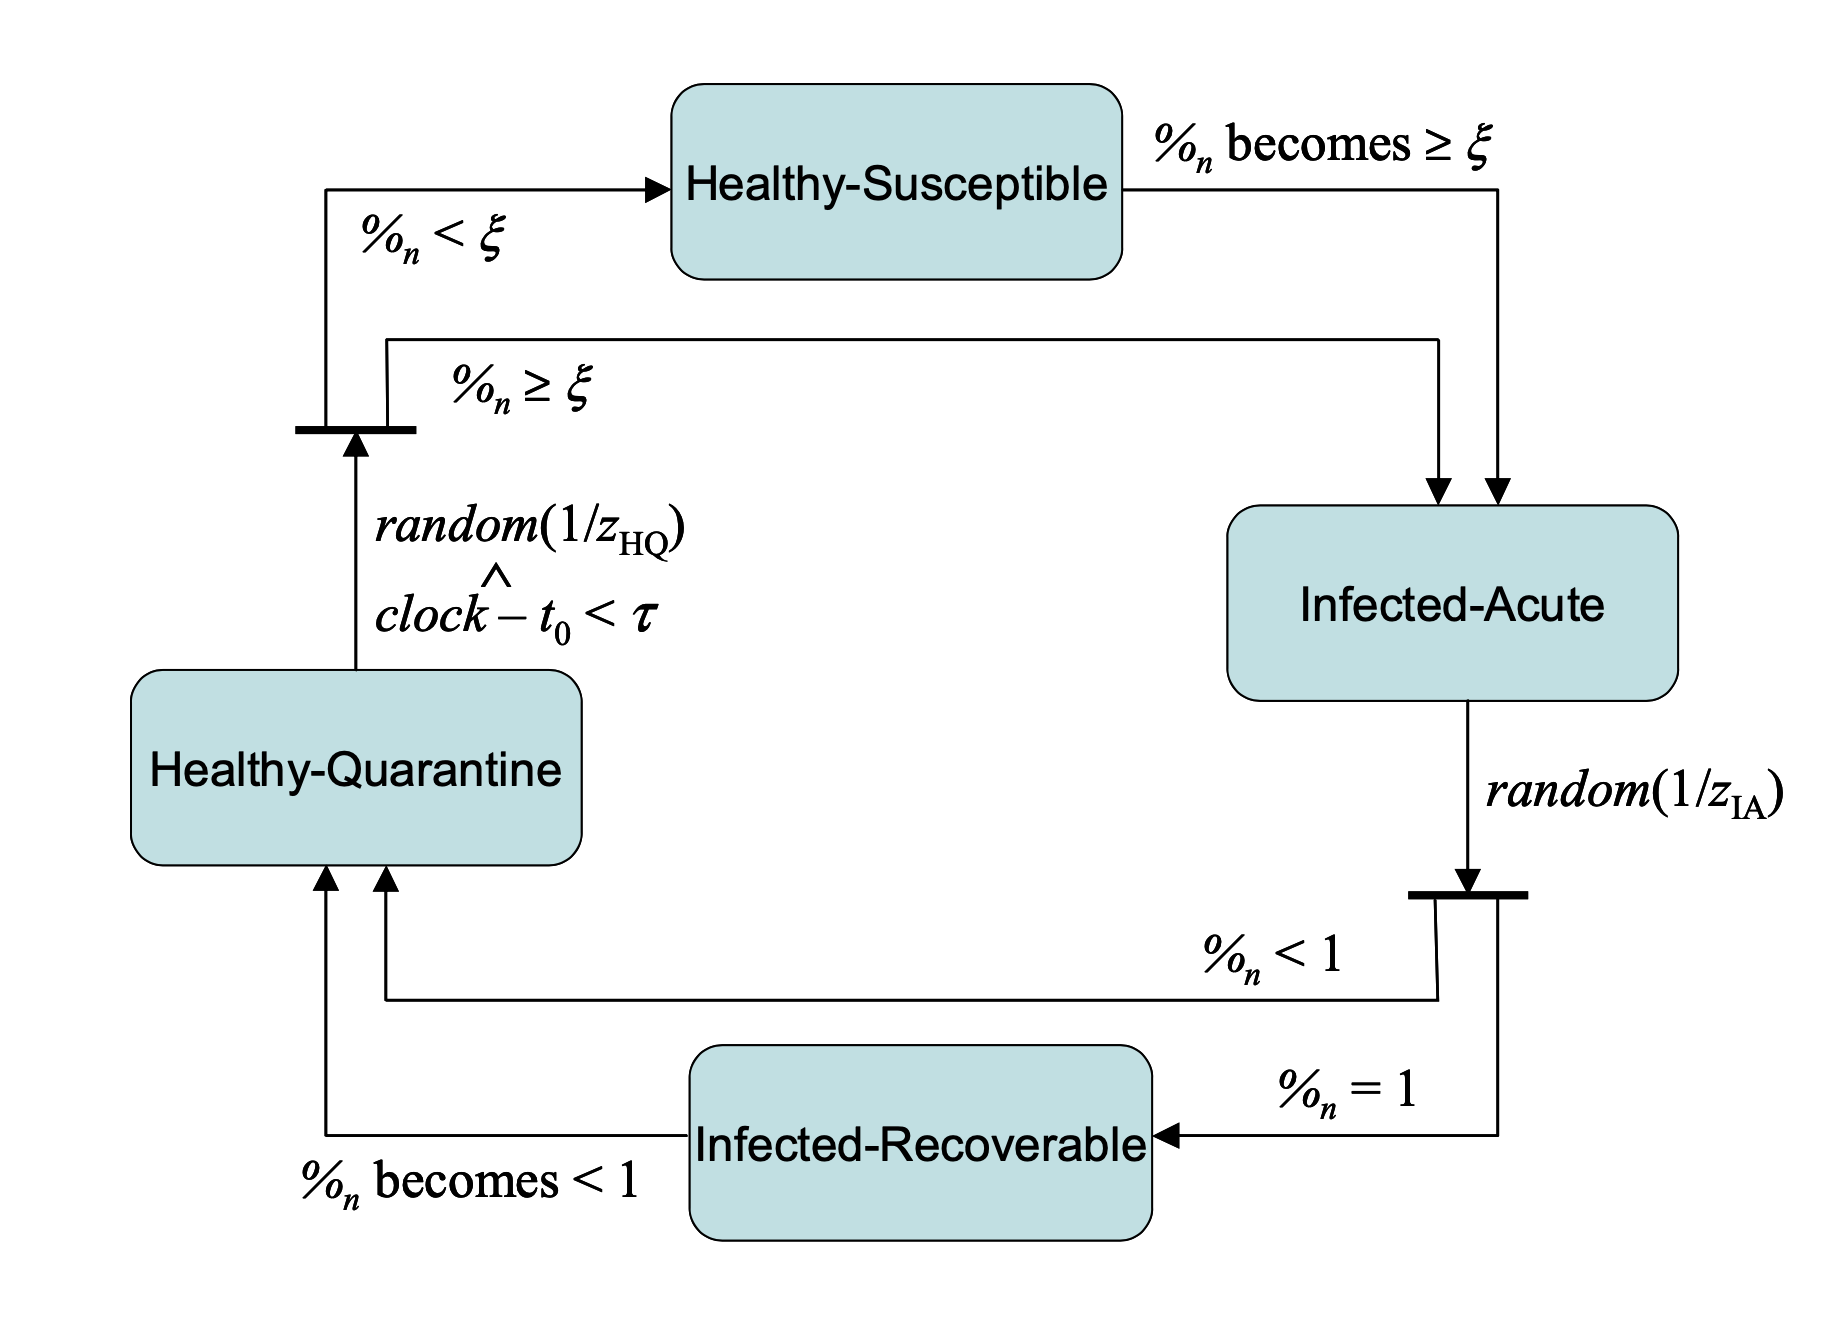
\includegraphics[width=11cm]{img/finite-state-at-node.png}
    \centering
    \caption{Finite state machine at node. Source: Mitigating Time-Constrained Stolen-Credentials Content Poisoning in an NDN Setting \cite{konorski2019mitigating}}
    \label{fig:finite-state-machine-jekon}
\end{figure} 
In Susceptible state nodes are healthly -- does not propagate infection -- but can get infection and change state to Acute; Acute nodes are infected -- does inflicts infection propagation -- and can switch state to Recoverable or Quarantine depending how many of their neighbors are infected; Recoverable nodes are infected, but can switch to Quarantine if some of their neighbor gets healthy; Quarantine nodes are healthly, and can switch state to Susceptible or Acute depending how many of their neighbors are infected. 
Nodes can get infected by either:
\begin{enumerate}
    \item external infection -- content publisher can always infect his home node, and then next nodes after fixed period of time.
    \item internal infection -- when the fraction of infected neighbors pass the $\xi$ treshhold, then the node gets infected. 
\end{enumerate}

At the beginning all nodes are healthly (distrust new content). When publisher wants to authenticate new content, he start the infection process. Initially he can infect only home node that is assigned by some external mechanism. Home node issue certificate that allows to infect next random node after some constant period of time. After that time, the publisher infect next node by showing the certificate signed by previous node. This process is then repeated until the network lead to the epidemic, or, the publisher, will be out of time with its stolen credentials. To give this process some momentum, we allow the nodes to infect each other by internal infections. That way, the publisher doesn't need to coordinate whole process until the epidemic, but just start the chain reaction with sufficient power (proofs-of-time) which will then turn into epidemic itself.

Internal infections works as follows: node $n$ in susceptible state, switch to acute state, by being infected by its neighbours $N_n$ only if the threshold $\xi$ gets reached by the fraction of its infected neighbors $\%_n = |I_n|/|N_n|$, where $|I_n|$ is the number of infected $n$'s neighbours and $|N_n|$ is the number of all $n$'s neighbours. To give some momentum both acute and quarantine state are introduced. The node in one of this states have to spend some random time in it before it can leave the state. Here the $random(1/Z_{IA})$ and $random(1/Z_{HQ})$ are introduced to denote the random period in which the node needs to spend in that state before evaluating its neighbours. $Z_{IA}$ dictate the number of cycles in acute state, where $Z_{HQ}$ do the same for quarantine state. Node in acute state, after the random period that on average take $\frac{Z_{IA}}{2}$ cycles leave its state. Depending on the $\%_n$ it switch either to recoverable -- if the $\%_n = 1$; or directly to quarantine -- if the $\%_n < 1$. In recoverable state the node is still infected, but as soon as one of his neighbours recover, it immediately switch to quarantine. Quarantine state is simillar to acute with one exception, node can be locked in this state if it gets immunized. The immunization is acquired after $\tau$ cycles from the first infection on the node. It works as a timeout, preventing from endemic state of the network. When the network stays in endemy for long time, it means that the publisher proof-of-time was to weak to reach epidemic. As we discussed earlier, there is no known analytical solution to such graph model, therefore it needs to be simulated on computer.

\subsection{Simulator}
We provide two simulators, first for visualization and second for fast calculations. Visualization simulator helps us better understand processes on graph, and find potential problems. Fast simulator allows us to perform many calculations on different input data in reasonable period of time. The source code for both simulators is available under this link \url{https://github.com/stasbar/ProofOfTime-Auth}. Both simulators are presented in Fig. \ref{fig:simulators}. Visual simulator is accessuble under \url{masti.stasbar.com}.
\begin{figure}[h!]
  \subfloat[Visual simulator]{
	\begin{minipage}[c][1\width]{
	   0.5\textwidth}
	   \centering
	   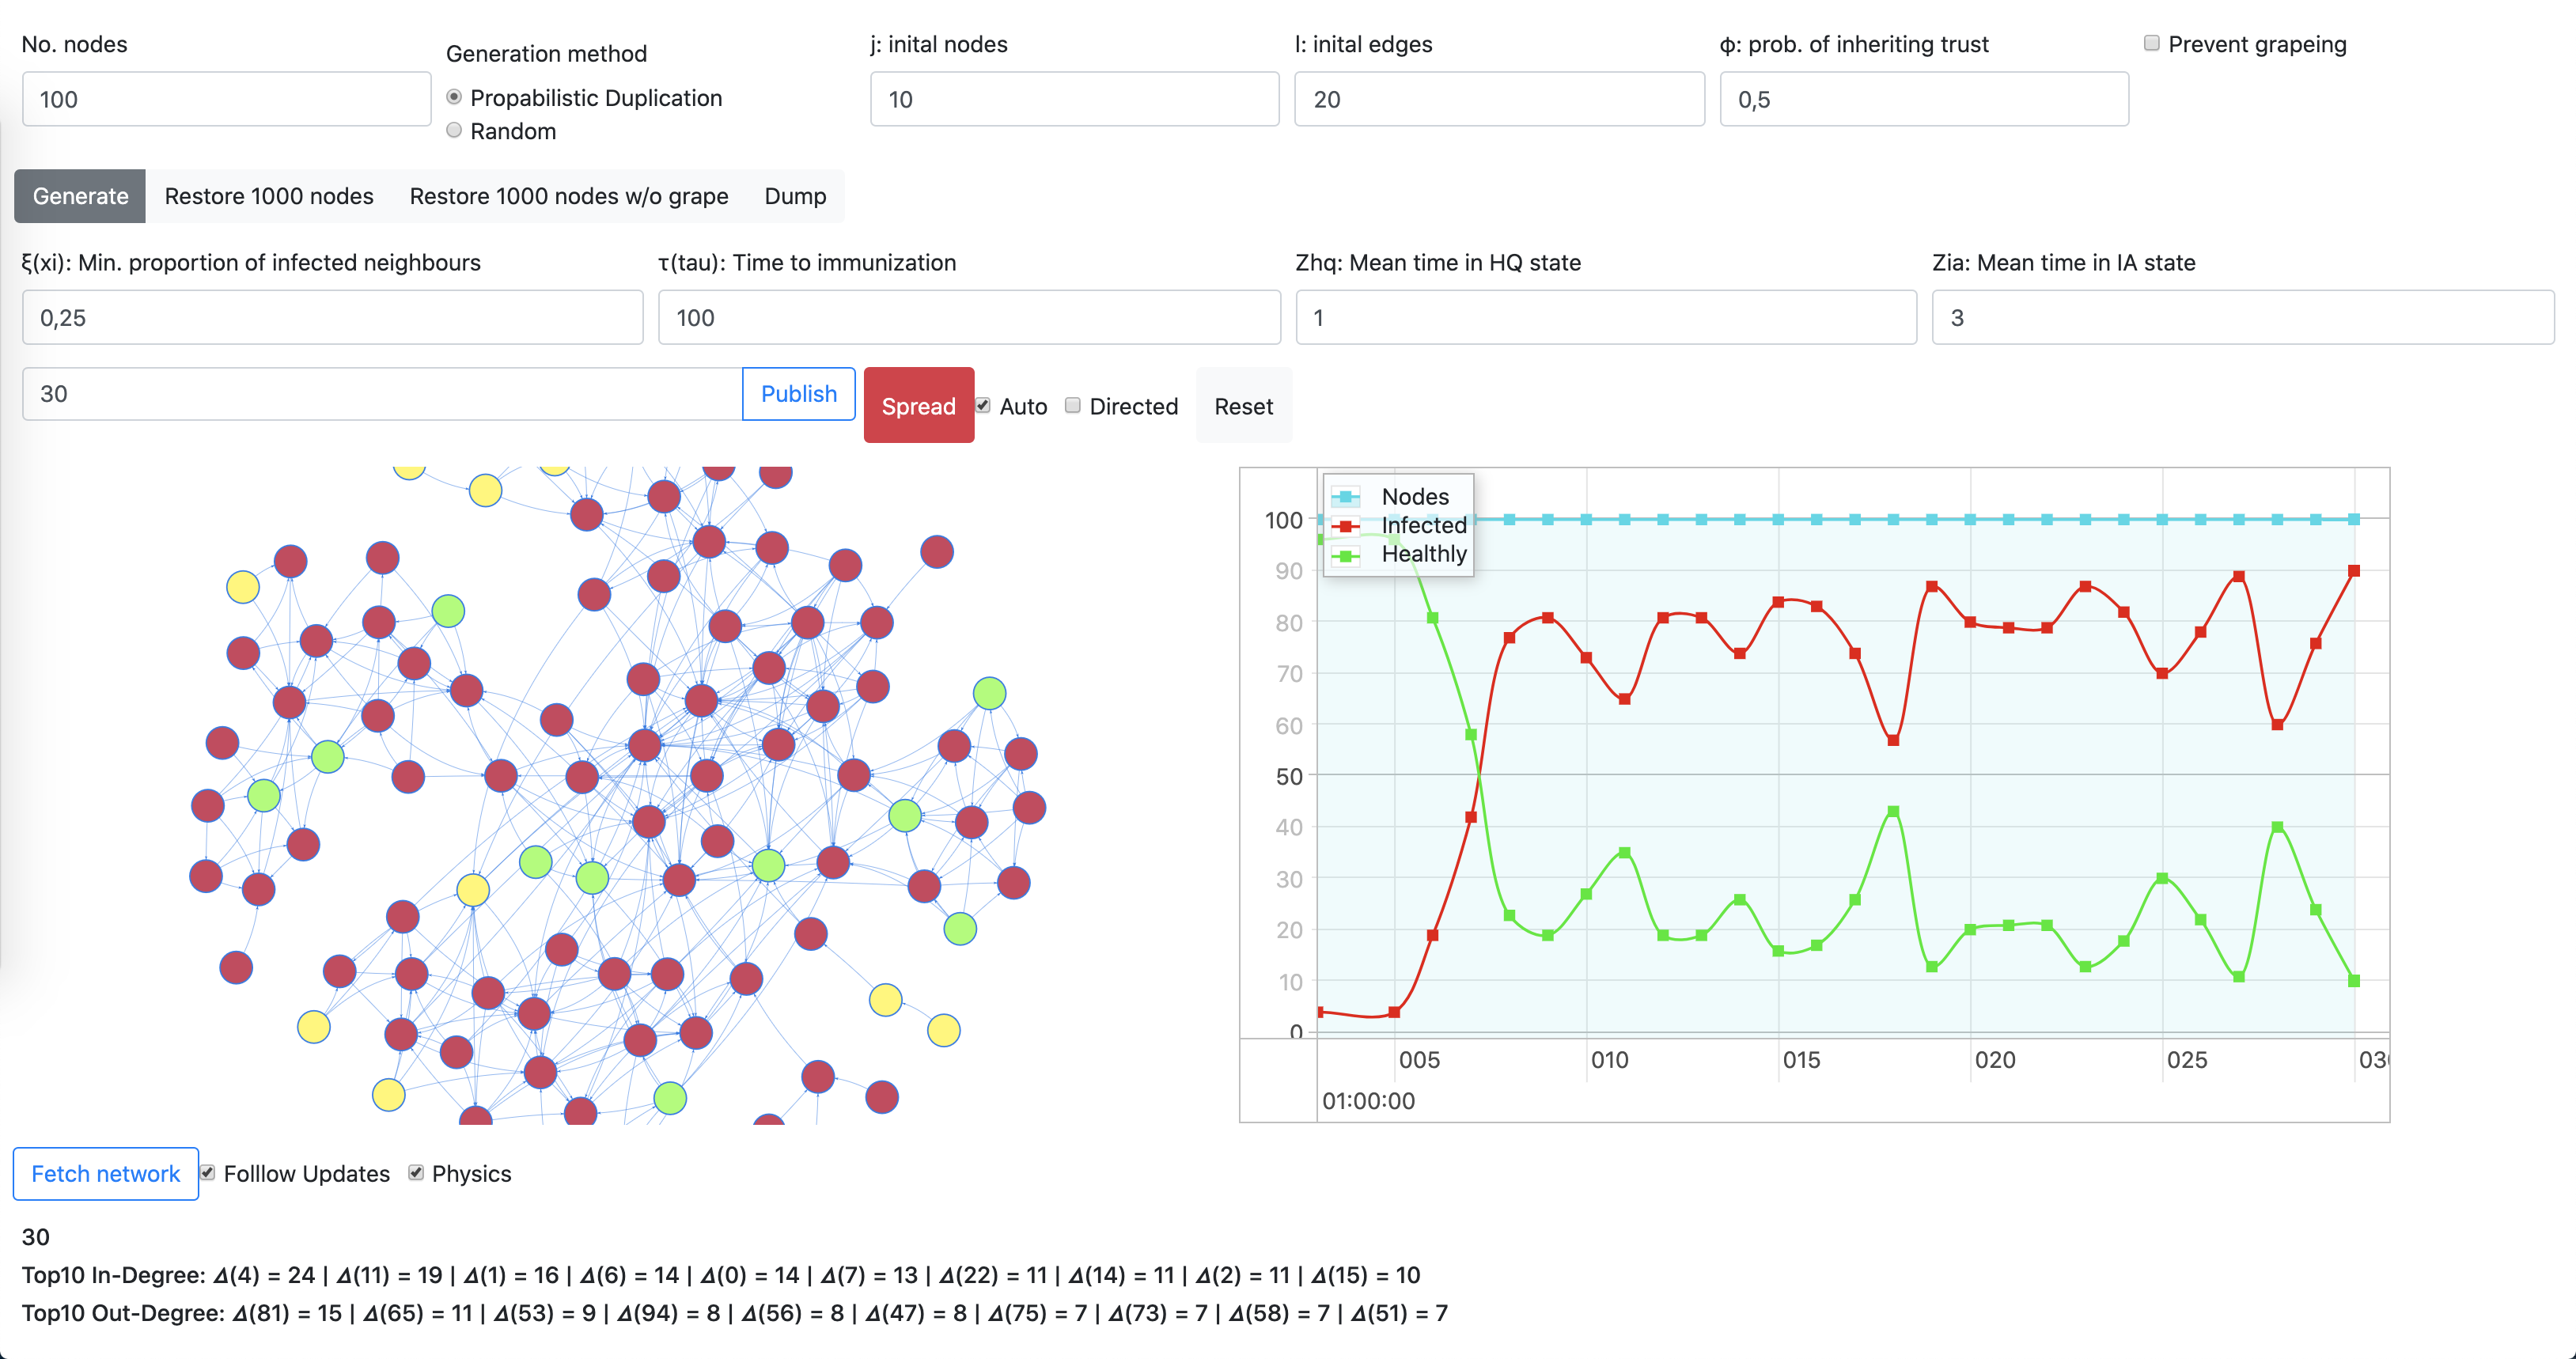
\includegraphics[width=1\textwidth]{img/simulator.png}
	\end{minipage}}
 \hfill 	
  \subfloat[Fast simulator]{
	\begin{minipage}[c][1\width]{
	   0.5\textwidth}
	   \centering
	   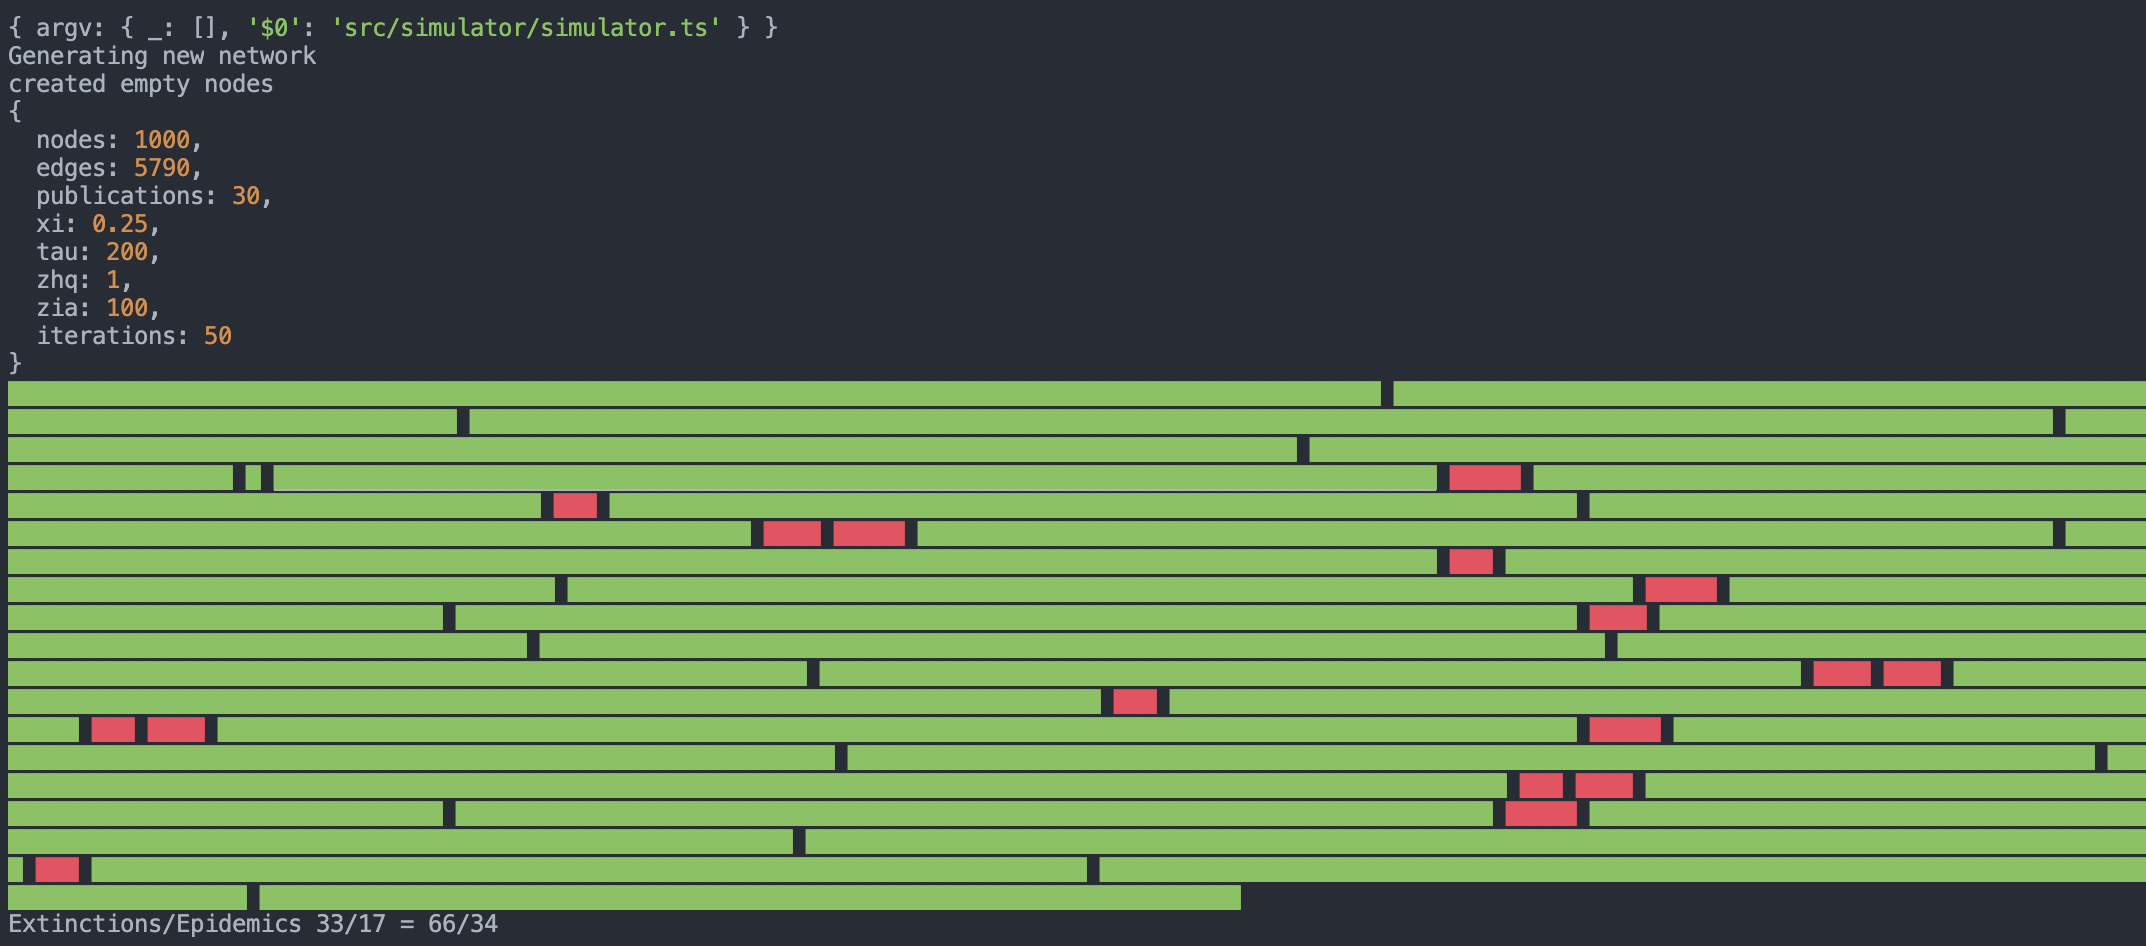
\includegraphics[width=1.1\textwidth]{img/fastsimulator.png}
	\end{minipage}}
\caption{Simulators preview}
\label{fig:simulators}
\end{figure}
Simulators allows us to generate the trust graph using 3 different generators: random, web of trust and probabilistic duplication discussed in Section \ref{trust-graph}; and customize the parameters: number of nodes, number of nodes and edges in initial kernel and $\phi$ -- used in web of trust and probabilistic duplication to customize the connections density. After the graph is generated we can save it and restore it -- that way we always work on the same graph during the research. 
When the graph is loaded, we can set the $\xi$, $\tau$, $Z_{HQ}$, $Z_{IA}$ and number of external infections or publications or proofs-of-time. 
Visual simulator provide us live preview of graph and chart during the infection process.  
Fast simulator print the results of simulations, green color indicate that the network ended in extinction state, red color indicate the epidemic state; length of the block indicate the number of cycles needed to reach the final state.

\subsubsection{Observations}
Running the visual simulation provide us some interesting feedback. We notice that there is some unfortunate graph and $\xi$ configuration that prevent whole network from reaching epidemic even with with strong proof-of-time i.e. a lot of external infections.
If in trust graph $G$ there exist defensive alliance $A \subseteq G$ of connected nodes $v \in A$, where each node $v$ is connected to less than $\xi * |N(v)|$ nodes outside the $A$, then such alliance prevent whole network from epidemic. If we assume $\xi = 1/4$ and graph structure visible on \ref{fig:defensive-alliance}a,
\begin{figure}[h!]
  \subfloat[]{
	\begin{minipage}[c][1\width]{
	   0.5\textwidth}
	   \centering
	   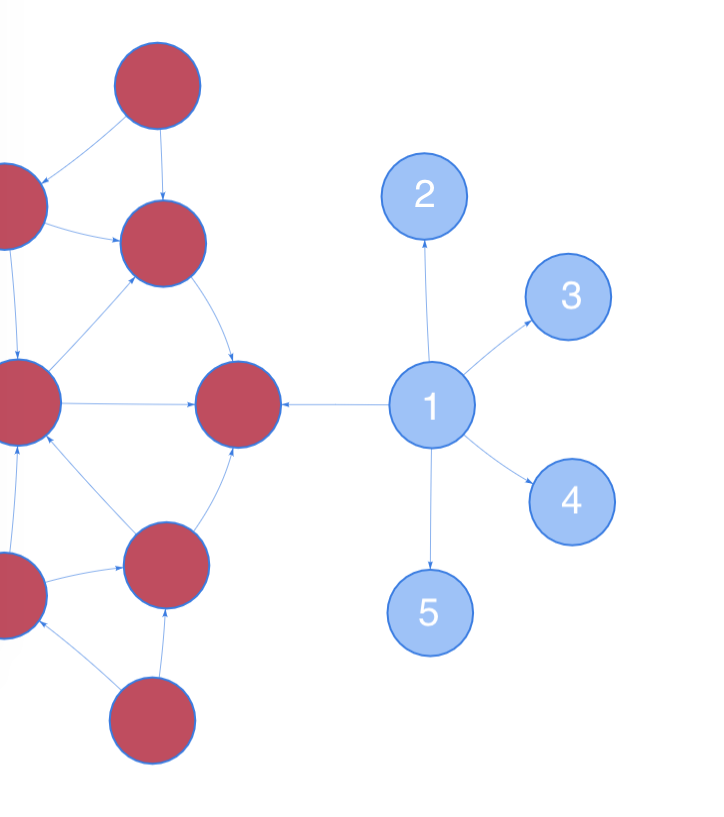
\includegraphics[height=0.7\textwidth]{img/offensive-alliance-numbered.png}
	\end{minipage}}
 \hfill 	
  \subfloat[]{
	\begin{minipage}[c][1\width]{
	   0.5\textwidth}
	   \centering
	   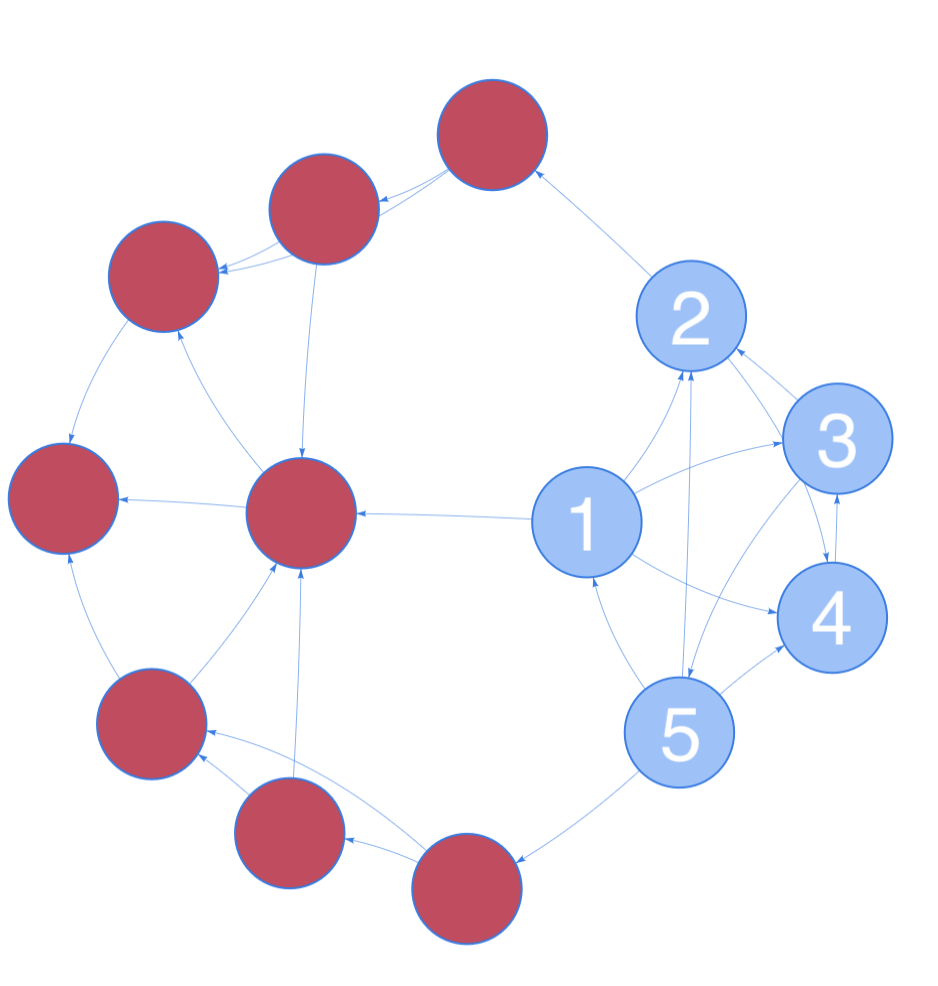
\includegraphics[height=0.7\textwidth]{img/offensive-alliance-clique-numbered.png}
	\end{minipage}}
\caption{Defensive Alliance}
\label{fig:defensive-alliance}
\end{figure}
then infected nodes (red) are not able to infect the healthy ones (blue), especially the $v_1$, which is the single node connected to the outside of $A$. It happens because the healthy node $v_1$ is connected to $\xi^{-1} = 4$ healthy nodes $\{v_2,v_3,v_4,v_5\}$ that are also part of $A$, so the one infectious node can not reach the $\xi = \frac{1}{4}$ threshold when there is already $\frac{4}{5}$ healthly nodes connected to $v_1$.
Let's take different graph where defensive alliance $A$ is connected to rest of the graph $G \setminus A$ through more than one node as shown in \ref{fig:defensive-alliance}b. Nodes from $A$ can not be infected since there is not enough connections from outside $A$ to reach the $\xi$ threshold. We define defensive alliance by \[\forall{v \in A}, \frac{|N(v) \cap A|}{|N(v)|} > 1 - \xi.\] 

The result is that rest of the network stays in acute state until the nodes connected to $A$ change their state to quarantine (notice that their $\%_n$ is less than 1), which then propagate on the rest on the network leading to extinction. 

Of course, we could generate network where such alliances are prohibited, but we previously assumed that the trust graph can have arbitrary structure, and the used generator is only the supposition. Lowering $\xi$ may be another option, but that way we speed up the infection process on whole network which is unwanted effect.

There is no known solution to finding defensive alliances or even answering question if there exist such one in polynomial time. Therefore the only way of finding the defensive alliance in graph is exhaustive search. The problem gets even worst if we assume that the network is open, and in any moment anyone can join or leave. 

\section{Consensus}
If we look at the problem from different perspective we notice that what we are trying achieve is to achieve consensus among all nodes about the decision if the content is legit or bogus. In graph infection algorithm, the consensus was dictated by the initial power of the chain reaction process. Too low power lead to extinction, high enough power lead to epidemic. Both epidemic and extinction can be considered consensus decision. In epidemic the whole network generates positive decision about the content authentication, while in extinction they decide not to trust it. 

% Very important chapter
If we evaluate Graph infection in terms of consensus problem, it turns out that it struggle with faulty nodes. In graph infection each node controls the time after the next propagation is allowed, if the node failed, it can allow immediate propagation or doesn't allow it at all. Additionally the consensus is not deterministic, there is no guarantee that with the initial conditions the network will reach the same final state for each iteration. Although the consensus finality is achieved using timeout (the $\tau$ specify the iterations after node gets immunization), the time to reach consensus is non-deterministic.

If we consider stronger form of faulty nodes called \textit{Byzantine failure}\cite{lamport2019byzantine} that allow nodes to act arbitrary, then such node can stuck in either healthy or infected state ignoring state of its peers, that way one single faulty node, can change the decision of non-faulty nodes. In consequence, it can prevent whole network from reaching extinction or epidemic.

We evaluate the algorithm using three known consensus requirements, which are: Validity, Agreement and Termination.
\begin{enumerate}
    \item Validity: any value decided upon must be proposed by one of the processes.
    \item Agreement: all non-faulty processes must agree on the same value
    \item Termination: all non-faulty nodes eventually decide.
\end{enumerate}
Validity and Agreement specify what must not happen, in distributed systems literature\cite{lamport1977proving} those are called safety property. Termination specify what must happen and is called liveness property.

We proved that in strong form of Byzantine-failure-node the protocol neither satisfy fault-tolerance nor safety. One single faulty node can prevent non-faulty nodes to decide on the same value--breaking the safety requirement using one single faulty node. Although liveness--eventual termination--is satisfied, the protocol should be disqualified since the eventual-termination is possible only to extinction state. We can say that the protocol can asymmetrically-terminate. In other words, we can not state that the protocol will eventually lead to either epidemic or extinction, we can only say that the protocol will eventually lead to extinction.

% Very important chapter
We don't claim that its impossible to form the graph infection algorithm that satisfy those properties. If the nodes would gain more awareness of the state of the network, they could detect faulty nodes and therefore become fault-tolerant.

There are variety of different consensus algorithms, they differ in terms of kind of node failure (Byzantine or not), synchrony (Asynchronious or Synchronous), number of tolerated failure nodes, authentication (if messages have to be signed by their authors), number of rounds to achieve consensus. Instead of solving our initial trust problem at the consensus layer, we propose solution that can be deployed on top of already existing consensus protocol. We search for protocol that work with Byzantine-fault nodes, because in internet level protocol managed by many organizations we can not assume that all nodes will act honesty. Additionally the protocol must allow open membership, the nodes should be able to easily join and leave the network supporting network decentralization. 

\section{Blockchain}
Consensus protocols that works with Byzantine-failure nodes and allow open membership are used in open blockchains. By open blockchain we understand the blockchains where nodes can freely join the network and participate in the consensus protocol. Examples of such blockchains are Bitcoin, Ethereum and Stellar. Bitcoin uses proof-of-work consensus algorithm where the computational power dictate the contribution into the consensus decision. Ethereum plans to switch to proof-of-stake consensus where the amount of cryptocurrency dictate the contribution into the consensus decision. Stellar uses federated byzantine agreement where the trust dictate the contribution into the consensus decision. Data stored in Blockchain is immutable, transparent and secure. Data types differ in different blockchains, but most of them store the transactions that update the global ledger. Some blockchains, like Ethereum also allows to store smart contracts\footnote{Scripts that are executed on virtual machines on all nodes, and uses blockchain as a persistent storage}. In our case we use blockchain to store proofs-of-time claims. Fortunately such claims can be embedded in most of the blockchains data types.

Let's imagine naive solution based on Bitcoin blockchain. The solution is naive because, proof-of-work has no practical application in our system. We can not base our system on the competitive consensus algorithms, especially on resource-constrained network devices. Nevertheless, the solution can be applied on any other consensus protocol, so we decide to explain it on the simplest and most commonly known one. 
Before we start to explain the algorithm, let's recall what we want to achieve. We want the end user, the content consumer to be sure about the content authentication. We achieve it by requiring the publisher to proof its access to private keys for long period of time, long enough so the malicious publisher can not afford to do that, while legit publisher can. We call those access proofs -- proofs-of-time. In graph infection algorithm the proof-of-time is denoted in sequential number of external infections. The publisher who is able to perform long enough proof-of-time, is able to create strong initial power of chain reaction, that will lead to epidemic, while the weak proof-of-time will eventually lead to extinction. 

In the blockchain solution, the simplest way to proof access to private-key in context to some content is to publish transaction from the publisher account to the content account. The content account, is the imagined account which address is hash of such content. The publisher account is the same key-pair used to sign the content in ICNetwork. The flow is shown in Fig. \ref{fig:distribution-flow}.
\begin{figure}[h!]
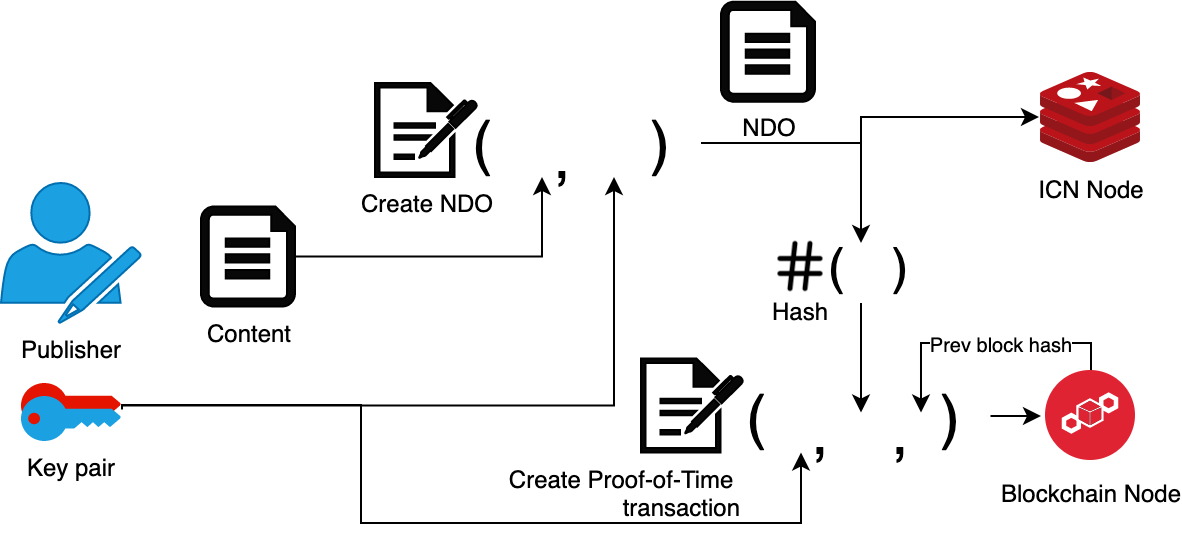
\includegraphics[width=9cm]{img/distribution-flow.png}
\centering
\caption{Flow of publishing content to ICN and proof-of-time to blockchain}
\label{fig:distribution-flow}
\end{figure} 
Strength of the proof-of-time is calculated by counting total number of transactions to the content hash address. Here we will use one of the most fundamental features in Bitcoin blockchain -- blocks. Block is a container holding bunch of transactions. Bitcoin is designed to produce new block every 10min on average, it is achieved by dynamic complexity of mining process. If we count each block where the transaction from publisher account to the content hash exist, we get the strength of proof-of-work that can be interpreted as sufficient to trust the content. This way, the proof-of-time is propagated not as a consensus, but as overlay structure on top of trusted neutral immutable database. 
As we mentioned earlier, the bitcoin and any other proof-of-work consensus is not suitable for our purposes


\section{Federated Byzantine Agreement}
We find Federated Byzantine Agreement (FBA)--and its blockchain Stellar Consensus Protocol (SCP)\cite{mazieres2015stellar}--the most suitable protocol for our needs. In contrast to proof-of-work, where computational power dictate the contribution to consensus, FBA is based on trust model. That way, it become lightweight and asymptotic resistant, meaning that the node consisting of large computational power does not gain any advantages in the consensus protocol. Instead the contribution value is determined by the node trustworthy--similarly to graph infection protocol. New node, joining the network, has no contribution to the protocol until someone trusted--start to trust it.
Blockchain like any other asynchronous distributed system, faces FLP\cite{fischer1985impossibility} impossibility trilemma---where only two of three properties can be achieved. Those properties are: Fault tolerance, Liveness and Safety. Most systems must be fault tolerance so the choice is left between Liveness and Safety. Safety guarantee state consistency across all nodes in the network. If nodes does not agree on some transaction, they will not split to two different states, but rather wait until the conflict is resolved. Liveness guarantee that the consensus will always terminate, and the system will always be available to new transactions. Choosing liveness over safety, when the conflict occurs, the ledger split to two different versions, until it's resolved, but in the mean time, it can process all new transactions. Most of the blockchain protocols chooses liveness, tolerating temporary partitioning. They argue that the time of the partitioning is short enough that the users expecting high credibility of the transaction can just wait--until the chance of shifting the state is acceptably small\footnote{In proof-of-work the chance of changing the state of some block gets smaller with the length of chain of the blocks attached to this block}. The conflict settlement is dictated, again, by computational power. The state which gets the fastest used as a previous block is considered winner. That way the system can guarantee permament availability, even with just one working node. 

Stellar on the other hand chooses safety over liveness. Once the state has been approved, it can not be changed. State gets approved if at least 66\% of the network agree on proposed state. This allows much faster confirmation times, in Stellar the ledger closes in about 5 sec. 
Stellar Consensus Protocol is based on Practical Byzantine fault tolerance (PBFT)\cite{castro1999practical}, and extends its functionality by allowing open membership, therefore promoting decentralization. In SCP each node pick its trusted set of nodes called \textit{quorum slice} (in which it is also \textit{ipso facto} a member). The \textit{quorum slice} should be different for each node, but naturally some nodes are more trustworthy, therefore are chosen more often in the quorum slices. Transitive trust for all node's \textit{quorum-slice} members, forms \texit{quorum}. For any two quorums, there must exist \textit{quorum-intersection} to prevent network partitioning. 

In non-federated byzantine agreement systems, the decision on some state proposal is determined by the majority of the nodes. Once the proposal gets accepted by quorum (majority of the nodes), the rest of the network can be sure that other proposals will fail, since they can't reach the quorum, since the nodes can't change their mind. That way the whole network converges to the final outcome.
In decentralized systems, where nodes can join and leave at will, its hard to know the total number of nodes in the network \texit{a priori}. Therefore it's hard to calculate the majority of the network. Additionally open systems can not rely on quanitive majority since this would open them to sybil attacks\footnote{In this attack single entity can join many nodes to the network that looks as indepenent units, therefore forcing decisions based just on majority number of nodes}. To solve this issue, FBA introduces the federated voting process that starts locally and expands until it reach whole network. To make it work, the local quorums must overlap with at least one node that will convey the voting decisions across different quorums. This property guarantee that if one quorum vote on some value P, the other quorum can not vote on not-P, because it includes some nodes from the first quorum that already voted on P.




When the nodes attend to agree on one version of the ledger, they start voting process inside their \textit{quorum slice}. And the process of approving the ledger is based on voting. 

Scalability is another feature where FBA shines. Nodes does not need to communicate with all other nodes in the network (like in other PBFT protocols) to achieve consensus, instead they need to communicate with their quorum-slice subset which is way more efficient, especially at internet level protocol.

% Possible remove
Also SCP does not introduce the concept of mining, therefore the incentive of joining the network as a validator is much smaller than joining as a miner, so the Stellar network is not as decentralized as e.g. Ethereum. We can find paper \cite{kim2019stellar} where authors shows that the whole Stellar network can stop, if only two nodes controlled by Stellar Foundation fail. David Mazières who designed the SCP, addressed this issue \cite{Safetyvs90:online}, and claims that the problem does no longer exist.

% Problems 
The problem arise, when such nodes (quorum intersection) are byzantine failed, lying about the decisions made on each quorums. In SCP whitepaper, there is assumption that the network is configured in such a way that even if the malicious nodes are removed from the network, it still holds quorum-intersection. If it does not hold, the network halts until the quorum-slices are reconfigured.
We can expect the network to form a connections where there always exist quorum-intersection because the internet--that we are designing the protocol for--itself satisfy such property.
How can we expect the network to form a connections where there always exist quorum-intersection ? 
There must be some mechanism to resolve the conflict

\section{Discission}
Proof of Elapsed Time (PoET)
%https://arxiv.org/pdf/1809.05613.pdf
%2) Proof of Elapsed Time (PoET): Proof of Elapsed Time is a consensus method proposed by Intel which works similar to PoW but with significantly lower energy consumption. In this method, miners have to solve a hash problem similar to that of PoW. However, instead of a competition between miners to solve the next block, the winning miner is randomly chosen based on a random wait time. The winning miner is the one whose timer expires first. The verification of correctness of timer execution is done using a Trusted Execution Environment (TEE) like Intel’s Software Guard Extension (SGX) [25]


\section{Modification}
%Disallow prepublishing
%Handle DoS other way than fee




In the figure \ref{fig:network-viz} 
\begin{figure}[h!]
\includegraphics[width=9cm]{img/stellar-network-viz.png}
\centering
\caption{Stellar public network structure source: https://stellarbeat.io}
\label{fig:network-viz}
\end{figure} 
we can see the Stellar public network graph. Nodes represent the validators - servers running Stellar Core software, and edges represents their quorum-slices. At the time of writing, the network consist of 59 Node validators held by 18 organizations, most of them located in USA, Europe, and East Asia.



\section{Federated Byzantine Agreement}
When we talk about trust graphs, blockchain and internet level protocols, we have to mention Federated Byzantine Agreement (FDA) which uses trust connections to secure its decentralized blockchain network. FDA was initially proposed for Stellar cryptocurrency, and its implementation is called Stellar Consensus Protocol (SCP). FDA is based on Practical Byzantine Fault Tolerance (PBFT) \cite{castro1999practical} used also in e.g. Ripple and Hyperledger. In PBFT nodes agree on the ledger using the voting process, once the 66\% of network agree on the state, the ledger is closed and can not be reverted. PBFT chooses Safety over Liveness, so the problem of blockchain partitioning does not exist. Once the transaction is approved by blockchain it can not change its state. Also the confirmation speed is much faster, in Stellar the ledger closes in about 3-5sec. What is most important it does not require mining for securing the network. Therefore it is asymptotic resistant, meaning that the node consisting of large computational resources does not gain any advantages in the network, especially can not proceed 51\% attack, that is possible in PoW protocols. 

In FDA each node chooses its own list of trusted peers. Those peers trust their trusted peers and so one (similarly as in our infection model), forming quorums. Each quorum must overlap with other quorum with at least one node. This model can hold up to 33\% Byzantine failure nodes. Additionally, FDA is much faster than bitcoin -- can process 200 transactions per seconds, and produces new block each 5 second. 


\section{Blockchain layer}
In our proposition nodes in the network plays two roles, ICN node where it participate in routing and content caching and as blockchain node where he participate in consensus and blockchain storage (see Fig. \ref{fig:layers}a). Not every node has to play two roles, the ones which are not connected to end-uses might not participate in blockchain network, since they don't get asked for content trustworthy. 
The blockchain layer could also be managed by completely different entities, separating transport layer from trust layer (see Fig. \ref{fig:layers}b). That way the ICN nodes could be abstracted from the trust network overhead introduced by trust system -- keeping them simpler and more reliable. Also the trust system would be more portable; it could be used in many different ICN solutions, and even in legacy systems since the trust does not depend on ICN but on the hash of the content and publisher credentials. That way the blockchain trust network could be hosted by more powerful devices, and 
\begin{figure}[h!]
  \subfloat[Combined layers]{
	\begin{minipage}[c][1\width]{
	   0.5\textwidth}
	   \centering
	   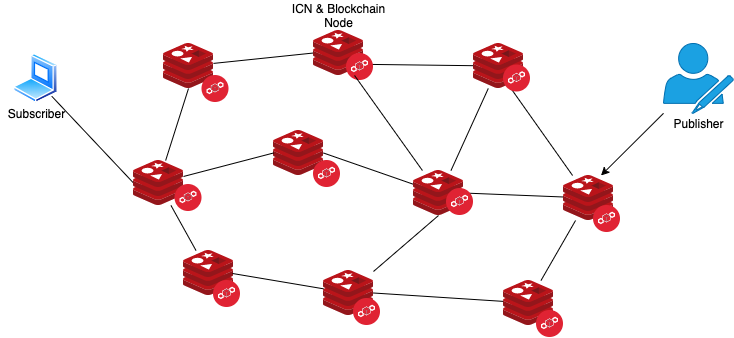
\includegraphics[width=1\textwidth]{img/combined-layers.png}
	\end{minipage}}
 \hfill 	
  \subfloat[Separated layers]{
	\begin{minipage}[c][1\width]{
	   0.5\textwidth}
	   \centering
	   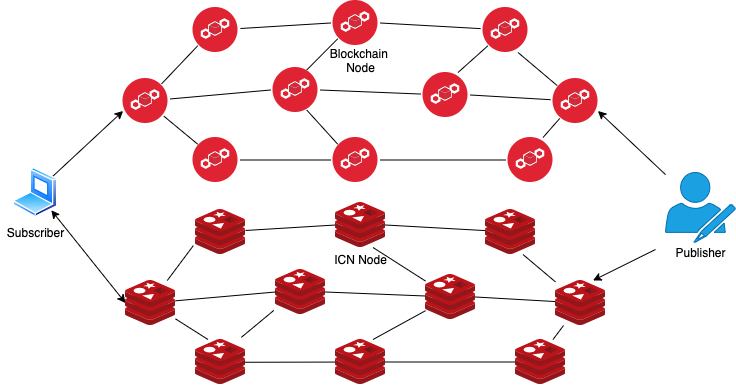
\includegraphics[width=1.1\textwidth]{img/separated-layers.png}
	\end{minipage}}
\caption{Layers}
\label{fig:layers}
\end{figure}


\section{Credibility Score}
In graph infection algorithm there are two states of content authenticity: authenticated or not-authenticated. We believe that this is limiting. Content like e.g. weather forecasting should not be authenticated for the same amount of time as online banking website. Therefore we propose more flexible model, where authentication can be acquired progressively via Credibility Score. Credibility Score mentioned in Section \ref{proof-of-time} increase authentication granularity. Pictures, music, movies doesn't require as much trust as websites where we enter our credentials and credit cards details. Different thresholds should be used for different content types. For example, if 3 trust thresholds are used: low, medium, high;


\section{Blockchain - Concrete solution}
We could use Bitcoin blockchain, or any other blockchain with constant time block creation, to persist proof-of-time claims. In Bitcoin each block is created in appx. 10min. We could take advantage of it, as a global, secure signing clock. Each new block has it's own unique hash, which can be used as a signing key. For our proof-of-time claims, or better we could persist our claims inside blockchain itself. Naive approach would be to send a empty (just fee) transaction from publisher account to hash of the content address. This way everyone can check, the history of hash of the content. Ensuring that it was proven by publisher for long enough. Of course this approach is conceptual. Bitcoin network is not suitable to operate in for network devices. Therefore we will outline the properties especially interesting in blockchain, and try to find out another blockhain or propose our own design. We consider Blockchain in first place, mainly because it's secure. Secure in terms of Byzantine Fault Tolerant system, but also as immutable storage. Not one can change the previously written data, without recalculating the proof-of-work puzzle, and overtaking rest of the network in computational power competition. This mechanisms works great for blockchains that servers store of value purposes. Our needs are completely different, we need a system that is asymptotic secure, so no (more powerful) node can overtake the whole network. That way, we lose the property of ~10min period ticking clock. We also can not incentivese nodes to behave honest by staking electrical power. We also need to get rid of fees since the Internet protocol on this level must be free. Therefore we need to protect from DoS attack in different way. Another important properties are openness and scalability. We need to design system that allow joining new participants and is highly scalable, otherwise we are limiting the protocol to special use cases, rather than global Internet protocol. Such software needs to operate on network devices which are resources constrained. Thus it needs to be lightweight, both in computational power and memory consumption.

Our solution to this problem is modification of \cite{konorski2019mitigating}, by adding Blockchain as a storage, and modifying consensus algorithm.

Each publisher who wants to publish the content to the network, must start with its home node. That node, create transaction in which he certifies the content proved by the publisher. Such certificate is then flooded to whole network, so they can update the current state of trust to the content. After some delay (clock tic), such node also create certificate in which he point to the one of neighbours node which can be infected next, where the publisher is also allowed to publish the content. The next node will accept the infection only if he is an home publisher, or if he is pointed as the next node by the previous node. Publisher show valid certificate (signed by previous node, and by himself - proving access to private key). Each node can create certification only once per content. 

That way, each node control the time of infection dissemination. If any node notice, that, the new certification was published earlier than previous certification + some fixed delay, it can assume that such node is cheating, and filter the certifications from such node.

Therefore we constructed new consensus algorithm where each node spread infection only if:
- didn't spread the infection for such content before
- previous time of infection was x time ago
- it is the home publisher or contains authorization token issued by some neighbour pointing to the node.

%TODO
//TODO



%TODO
//TODO

\section{Fusion - Graph infection blockchain based scheme}
We notice that, the chain of approval can be threat like a blockchain. Consensus mechanism here is based purely on each node. Each node control the time delay of the next block. If some node block the transaction, or sends it faster than designed (malicious actor), we can distrust that node. Each external publication create next block. Publisher is responsible for extending that chain to the length of acceptable trust to that content.

%TODO
//TODO

\section{Discussion}

\bibliographystyle{plain}
\bibliography{refs}

\end{document}

